%           %experimenting with svn-multi

\svnkwsave{$RepoFile: siminos/froehlich/flow.tex $}
\svnidlong {$HeadURL$}
{$LastChangedDate$}
{$LastChangedRevision$} {$LastChangedBy$}
\svnid{$Id$}

    \ifarticle
\begin{abstract}
    \else
\chapter{\CLf}
\label{chap:CLF}
\begin{quote}
{\bf Abstract:}

    \fi %end of article switch


    {\color{red}
%Stefan, write this: often! this might be the only part
%of this text that most people glance at.

%PC 2010-09-30: planted an error into the abstract, just to see how
%   often do you edit it.


When a dynamical system has a continuous symmetry, it is possible to exploit this symmetry to reduce the system to an equivalent simpler system. One methods for doing this is Cartan's \mslices. In this paper we investigate how the \mslices\ can be applied to linear subspaces. There are two main obstacles to using a subspace for the \mslices: the slice has to interesect every group orbit in order to be valid for the entire state space and the \mslices\ potentially introduces singularities into the flow. We show that any point in the state space can be rotated into these linear subspaces, guaranteeing they can be used for the entire state space and that singularities introduced into the system by the method of slices correspond to simple jumps in the reduced space and do not cause any actual difficulties. Throughout this paper we focus on $\SOn{2}$ symmetries, using the \cLe\ as a simple example. In addition we show that if the symmetry is a product of $\SOn{2}$ symmetries acting on distinct coordinates of the state space, then it is sufficient to consider each $\SOn{2}$ action independently.

    }
    \ifarticle
\end{abstract}
    \else
\end{quote}
    \fi %end of article switch



\section{Introduction}
\label{sect:intro}
Many papers have been written about using symmetries to help understand different fluid flows. This has been done for fluid flows such as the \KS\ equations \rf{ku,siv}, the plane-couette flow \rf{Visw07b,GHCW07,HGC08,HalcrowThesis}, and a pressure driven flow through a cylindrical pipe \rf{Wk04,Kerswell05}. These systems are relatively simple systems that experience turbulent flow. The hope is that understanding these simpler systems will provide a better understanding of turbulence.

Rotational and translational symmetries appear in many fluid flows. An example is a cylindrical pipe \rf{Wk04,Kerswell05}. If you rotate the pipe around its central axis it does not change the system. Any flow through the pipe can be rotated around the central axis and the resulting flow is still valid. These rotations of the pipe are an example of a continuous symmetry.

Several methods exist for exploiting a continuous symmetry of a system. The most prominent method is to rewrite the system in terms of a Hilbert basis for the symmetry. The state space coordinates are replaced by polynomials that are invariant under the action of the symmetry group. The polynomials are chosen to form a basis for the space of all invariant polynomials but are related by relations called syzygies \rf{DasBuch}. Hilbert bases work very well for low dimensional systems, but the number of basis polynomials and the difficulty to calculate them greatly increase with the dimension of the system and they are infeasible to calculate for the high dimensional (possibly infinite dimensional) flows encountered in fluid systems. Cartan's \mslices\ \rf{CartanMF} provides a less computationally intensive method for these high dimensional systems. In the \mslices\ the dynamics of the is system is replaced with an equivalent system on a subspace of the state space. This method is already being employed to reduce symmetries in various fluid flows \rf{SiminosThesis,rowley_reconstruction_2000,rowley_reduction_2003}.

One simple choice of the subspace is a hyperplane. This paper will investigate this use of hyperplanes for the \mslices\ with an emphasis on $\SOn{2}$ symmetries since these appear in many fluid flows (specifically the \KS\ equations, plane-couette, and pipe flows mentioned earlier). These linear slices are used in \rf{SiminosThesis,rowley_reconstruction_2000,rowley_reduction_2003} to reduce the dynamics of fluid flows.
There are two main obstacles to being able to use a subspace for the \mslices: every point must be rotatable into the slice and the \mslices introduces singularities into the flow.
Locally any point is rotatable into a linear slice, and ref. \rf{rowley_reconstruction_2000,rowley_reduction_2003} demonstrate that this is true globally for certain state spaces. This paper provides a more general proof that is applicable to more state spaces than that of \rf{rowley_reconstruction_2000,rowley_reduction_2003}.

The second difficulty with the \mslices\ is that it can introduce singularities into the flow. One method of handling this to do as in \rf{SiminosThesis} and choose the subspace so that these singularities do not occur. This can lead to complicated subspaces being used for the symmetry reduction. While linear slices will in general experience these singularities, we show that in the case of a $\SOn{2}$ symmetry, and in general for `well-behaved' symmetries, these singularities correspond to nothing more than an instantaneous jump in the trajectory in the linear slice that is easily calculated.

Many fluid flows have symmetry groups which are the product of $\SOn{2}$ symmetry groups acting on distinct coordinates of the state space. We demonstrate that when using linear slices for these symmetry groups it is sufficient to consider each $\SOn{2}$ action seperately.

Throughout this paper the \cLe\ \rf{GibMcCLE82} will be used as an example because they posses a simple $\SOn{2}$ symmetry on which the method of slices can be done. The state space of the \cLe\ is only 5-dimensional, but the method is the same regardless of dimension and to understand how it works it suffices to use a simpler system.

Working with symmetries requires some background and the beginning part of this paper is devoted to building up the knowledge necessary to understand what a symmetry is and how it can be used. We follow this by proving some important results for linear slices and then close with a short section on how the \mslices\ can be used to find invariants of a symmetry. This paper draws heavily from the teachings of Chaosbook.org\rf{DasBuch} and makes use of its notation.

     \PC{
   When you write
   a project report or a research article, you always write abstract, introduction
   and conclusions first, and then keep rewriting them often.
   They are the most important parts of the text, as that is
   for most people only parts they will look at.
   }

    %
    \Private{ % subversion label pages
$\footnotemark\footnotetext{{\tt \svnkw{RepoFile}}, rev. \svnfilerev:
 last edit by \svnFullAuthor{\svnfileauthor},
 \svnfilemonth/\svnfileday/\svnfileyear}$
    } % end \Private{

\noindent {\bf Acknowledgments.}
This report is written in collaboration with
% E.~Siminos and
P.~Cvitanovi\'c.
S.F. work was supported by the National Science Foundation
grant DMR~0820054 and a Georgia Tech President's Undergraduate
Research Award.
P.C. thanks Glen Robinson Jr. for support. 	

    \ifarticle
    \else

\section{Linear stability}
\label{sect:stability}
%\PC{Write up here the general text on stability, following \refref{DasBuch},
%\\
%\wwwcb{/chapters/stability.pdf}
%    }

When studying the trajectories of a flow, it is useful to
know how small neighborhoods of points are transported by the
flow. Understanding this gives us a better idea of how

Consider the displacement of an infinitesimally close
neighbor $x+\delta x$. Taylor expanding the flow equation
$\dot x = \vel(x)$ we find that
\beq
\dot x + \dot{\delta x}=v_i(x+\delta x) \approx v_i(x)+\Mvar \delta x
\eeq
where we shall refer to the matrix of velocity gradients
\beq
\Mvar_{ij}(x)=\frac{\partial v_i (x)}{\partial x_j}
\ee{SF:stabMat}
as the \stabmat.
In our first attempt to understand the dynamics of the flow,
we examine the \eqv\ of the system by finding this \stabmat\
$\Mvar$. For the \cLe\ it is the $[5\!\times\!5]$
matrix of velocity gradients,
                                                    \exerbox{exer:StabmatCLf}
\beq
  \Mvar =\left(\barr{ccccc}
    -\sigma    	& 0 		& \sigma & 0    &  0 \\
	0 	& -\sigma       & 0      & \sigma   &  0 \\
	r_1-z  &     -r_2      & -1     & -e & -x_1 \\
	r_2     & r_1-z       	& e  	& -1       & -x_2 \\
	y_1     & y_2           & x_1    & x_2      & -b
    \earr\right)
\eeq
As explained in ChaosBook.org\rf{DasBuch}, a \stabmat\
describes the instantaneous rate of shearing of the
infinitesimal neighborhood of $x(t)$ by the flow. That is, it
describes how quickly points initially very near to $x(t)$ will
diverge away from / converge to it in time. Matrix $\Mvar$ is an important
tool which we will use in what follows.

\subsection{\jacobianM}

We start by a discussion of the stability of \eqva\ and \po s,
and postpone the discussion of the stability of \reqva\ and \rpo s,
quintessentially continuous symmetry effects, to \refsect{SF:rpos}.

Consider the trajectory of a  neighbor infinitesimally close
to $\xInit$. Taylor expanding a finite time flow, we find that
\[
f^t(\xInit +\delta x) \approx f^t(\xInit)+\jMps^t(\xInit)\delta x,
\]
where
\beq
\jMps^t(x)_{ij}=\frac{\partial x_i(t)}{\partial x_j}
\ee{SF:jacMat}
 is
the \jacobianM. This means that up to the linear term the
neighborhood is transported by $\delta x(t)=\jMps^t(\xInit)\delta
\xInit$. This means that how nearby trajectories separate or
approach each other is dependent on the eigenvectors and
values of the \jacobianM.

The \jacobianM\ also maps the initial, Lagrangian coordinate
frame to the Eulerian coordinate at time $t$,
\beq
\velField{\ssp(t)}=\jMps^t(\xInit) \velField{\xInit}
\,,
\ee{JacobVeloc}
see \refexer{traLocEigFr}.
    \PC{remember to move \refexer{traLocEigFr}
    and its solution into ChaosBook. Currently it
    appears too early, search for ``traLocEigFr.''
    }

The methods of calculating the \jacobianM\ are discussed in ChaosBook.org\rf{DasBuch} where it is shown that the \jacobianM\ matrix is related to the stability matrix by $\frac{d}{dt} \jMps^t(x)=\Mvar (x) \jMps^t(x)$ or equivalently $\jMps^t(\xInit)= \texttt{T} e^{\int^t_0 d\tau \Mvar (x(\tau))}$, where \texttt{T} stands for a time-ordered product. When using a numerical routine to integrate the equations of motion, using a discrete approximation of either of these two formulas requires minimal additional programming effort.

% PC 13jul2010
\exercise{Transport of local eigenframes.}{     \label{traLocEigFr}
%    \toCB
\noindent (a)
Derive \refeq{JacobVeloc}.
(b)
More generally, consider the
eigen\-vectors $\jEigvec[j]$ of $\jMps^t(\ssp)$
(sometimes referred to as `covariant Lyapunov vectors,'
or, for \po s, as `Floquet vectors')
\index{covariant Lyapunov vector}
\index{Lyapunov!covariant vector}
\beq
\jMps^t(\ssp)\, \jEigvec[j](\ssp(t))
   = \ExpaEig_{j}(t) \,\jEigvec[j] (\ssp(t))
\,,
\ee{finTimeEigs}
and show that a time $t'$ later they are transported into
eigenvectors $\jEigvec[j](\ssp(t+t'))$ of
$\jMps^{t+t'}(\ssp)$.
\authorPC{2010-07-12}
    }% end \exercise{Transport of local eigenframes.


\solution{traLocEigFr}{Transport of local eigenframes.}{
\noindent (a)
Consider two points that are an infinitesimal time apart along a trajectory:
$\delta \xInit
  = \flow{\timeStep}{\xInit}-\xInit \approx \velField{\xInit}\timeStep$.
As $\flow{t+\timeStep}{\xInit} =
\map^t \circ \flow{\timeStep}{\xInit}=\map^{\timeStep} \circ \flow{t}{\xInit}$,
we have
$\flow{\timeStep}{\map^t(\xInit)}=\flow{\timeStep}{\ssp(t)}
\approx x(t) + \velField{\ssp(t)} \timeStep$ and
$\flow{t}{\flow{\timeStep}{\xInit}}
=\flow{t}{\xInit+\velField{\xInit} \timeStep}
\approx \flow{t}{\xInit} + \jMps^t(\xInit) \velField{\xInit} \timeStep$.
Putting these two equations together we get the desired
\refeq{JacobVeloc}.

\noindent (b)
Predrag: I am not sure that this statement is correct, please
prove or disprove. Basically, check that \refeq{SF:transpEigPO}
is true for any orbit, not only \po s.

A tangent subspace $T\pS^{(i)}$ of the \statesp\ is said to be {\em covariant} if
\beq
T\pS^{(i)}(\ssp(t)) = \jMps^t(\xInit) T\pS^{(i)}(\xInit)
\ee{SF:covSubsp}
This definition also applies to covariant vectors, if $T\pS(i)$ is one-dimensional.
Covariant subspaces
are co-moving with the tangent flow.
\authorSF{2010-07-??}
    }% end

\subsection{\Eqva}

An \eqv\ $\EQV{}$ is a point $\ssp_{\EQV{}}$ for which the
velocity field of an ordinary differential equation
$\dot{\ssp} = \vel(\ssp)$ is zero, $\vel(\ssp_{\EQV{}})=0$. These
are points where the flow does not move, and if it reaches an
equilibrium, the flow remains there. For the \cLe\, the
origin $\EQV{0}=(0, 0, 0, 0, 0)$ is always an equilibrium
point, but there are two more families of equilibrium when
both $r_2 + e=0$ and $r_1>1$. If we could set on of these
{\em infinitely precisely} as the initial point of the flow,
instead of seeing the messiness of \reffig{fig:CLEx1x2z}, we
would stay at this single point for all times. In any
simulation, for unstable \reqv\ the (finite precision)
trajectory eventually leaves this point.
                                                    \exerbox{exer:EquiCLe}

% \subsection{Stability of \eqva}

At an equilibrium, the flow manages to stay at a single
point, but what if we start at points near the equilibrium? Will
they collapse into the equilibrium, or will they diverge away
from it? In order to answer this, we find and examine the
eigenvalues and eigenvectors of \Mvar\ evaluated at the
equilibrium $\EQV{0}$, the origin.
                                                    \exerbox{exer:EigenE0}
For the \cLe\, we find that the eigenvalues are
        \PC{ChaosBook convention is to order eigenvalues
        from most positive (unstable) to the most negative,
        that is why I renumbered them. Try to follow that
        everywhere. Replace complex eigenvectors by the real,
        imaginary parts, as that is what you actually use - I
        did this in \refeq{eigVecQ1}. I might have introduced
        errors in renumbering them, so trust your own
        computations, especially regarding the
        \reffig{fig:CLEE0} comments.
        }
\beq
\begin{split}
\lambda_{1,2} &=11.8277 \pm 0.062985 i\\
\lambda_{3,4} &=-22.8277 \pm 0.037015 i\\
\lambda_5 &=-2.66667\\
\end{split}
\eeq
with the associated eigenvectors
    \PC{\label{suspectEigVecs}is suspect:
    real, im parts seem interchanged in $e_1$?}
\bea
e_{1} &=& e_2^* =(0.001321+0.4581 i, 0.4581-0.001321 i, i, 1, 0)
\label{suspectEigVecs}\\
e_3 &=& e_4^* = (0.002249-0.7795 i, -0.7795-0.002249 i, 2.8421+i, 1, 0)
\continue
e_5 &=& (0, 0, 0, 0, 1)
\,.
\nnu
\eea
By examining the eigensystem, we can get a sense of what
happens to points near the equilibrium $\EQV{0}$. The
numerical values of the real parts of the eigenvalues
determine how quickly the flow will converge onto or diverge
away from the equilibrium. For a positive real part the flow
will diverge, and for a negative real part it will converge.
Complex eigenvalues also indicate that the motion will be
spiraling.

For the \cLe\ equilibrium $\EQV{0}$, the values of the
imaginary parts are orders of magnitude smaller than the real
parts, so that there will be very little spiraling. The large
values of the real parts tell us that the flow will
diverge/converge from the equilibrium very quickly.
                                                    \exerbox{exer:PlotEigenE0}

To illustrate this, we plot the eigenvectors (as real and
imaginary parts) and the flow at initial points very close to
$\EQV{0}$. The two real vectors (corresponding to a single
complex eigenvector) define the plane in which the flow will
spiral. We initiate the flow very close to $\EQV{0}$ at a
point along one of these vectors. In \reffig{fig:CLEE0},
we can see that for the vectors with a very small imaginary
part and a positive real part, the flow does not spiral
noticeably and that it diverges away from the equilibrium very
quickly.


\subsection{\Po s}{
\label{sect:SFpos}

We can extend this analysis of linear stability to not only
work for single points, but also allow us to study the
dynamics of the system near periodic orbits.

Let $p$ be a prime cycle, $\ssp \in M_p$ be any point on the
cycle, $\period{p}$ the period of the cycle and
$\jMps_p\left(\ssp\right) = \jMps^{\period{p}}(\ssp)$ be
the {\jacobianM} for a single transversal of the cycle.
The {\jacobianM} for the $r$th repeat of the cycle is then
$\jMps^{r
\period{p}}\left(\ssp\right)=\jMps^{\period{p}}\left(f^{\left(r-1\right)
\period{p}}\left(\ssp\right)\right) \cdots
\jMps^{\period{p}}\left(f^{\period{p}}\left(\ssp\right)\right)\jMps^{\period{p}}\left(\ssp\right)
=\jMps_p\left(\ssp\right)^r$
This means that it suffices to only look at prime cycles when
considering the {\jacobianMs} of periodic orbits.

Next consider the {\jacobianM} of a prime cycle $p$.
Using what we know from Jacobians,
$\delta \ssp \left(t+\period{p}\right)
=\jMps_p\left(\ssp\right)\delta \ssp\left(t\right)$
so after traveling once around the cycle, it contracts along
the directions of the Floquet vectors with Floquet
multipliers of magnitude less than 1 and expand in the
directions of Floquet vectors with Floquet multipliers of
magnitude greater than 1.

Now this only tells us the rate of contraction and expansion
as the cycle is traversed, starting at a point $\ssp$, it
would be nice to now how it behaves as it traverses every
part of the cycle.

The value of $\jMps_p\left(\ssp\right)$ depends on the point
on the periodic orbit chosen, but, as we shall show, the
Floquet multipliers are independent of this selection. To see
this, let $\ssp$ be any point on the cycle and
$\jEigvec[j]\left(\ssp\right)$ be a Floquet vector of
$\jMps_p\left(\ssp\right)$ with Floquet multiplier
$\ExpaEig_j$. Consider another
point  $\ssp'=f^t\left(\ssp\right)$, $ 0 < t < \period{p} $
on the periodic orbit. $\jMps^{\period{p} +t}=\jMps^{t+\period{p}}$,
{\jacobianMs} are multiplicative along the flow:
\bea
\jMps^{\period{p}+t}\left(\ssp\right)
&=&\jMps^{\period{p}}\left(f^t\left(\ssp\right)\right)\jMps^t\left(\ssp\right)
=\jMps_p\left(\ssp'\right)\jMps^t\left(\ssp\right)
\continue
\jMps^{t+\period{p}}\left(\ssp\right)
&=&\jMps^t\left(f^{\period{p}}\left(\ssp\right)\right)\jMps^{\period{p}}\left(\ssp\right)
=\jMps^t\left(\ssp\right)\jMps_p\left(\ssp\right)
\,,
\nnu
\eea
and
\bea
\jMps_p\left(\ssp'\right)\jMps^t\left(\ssp\right)\jEigvec[j]\left(\ssp\right)
&=&\jMps^t\left(\ssp\right)\jMps_p\left(\ssp\right)\jEigvec[j]\left(\ssp\right)
    \continue
&=&\jMps^t\left(\ssp\right)\left(\ExpaEig_j \jEigvec[j]\left(\ssp\right)\right)
=\ExpaEig_j \left(\jMps^t(\ssp) \jEigvec[j](\ssp)\right)
\continue
\jMps_p\left(\ssp'\right) \jEigvec[j]\left(\ssp'\right)
&=& \ExpaEig_j
\jEigvec[j]\left(\ssp'\right)
\,,
\label{SF:transpEigPO}
\eea
where
$\jEigvec[j]\left(\ssp'\right)
 = \jMps^t\left(\ssp\right)\jEigvec[j]\left(\ssp\right)$
 is the $\jMps_p$ eigenframe transported for time $t$
 along the $p$ orbit.
So $\ExpaEig_j$ is a Floquet multiplier for
$\jMps_p\left(\ssp'\right)$ too.
    \fi %end of article switch


\section{Dynamical system}

We begin with a very brief discussion of dynamical systems.

A deterministic dynamical system is an abstract space $\pS$, called the state space, along with a rule for how trajectories on the space progress in time. We are concerned with applications to fluid flows, and as such we will only be concerned with systems where M is a manifold (locally it looks like $\mathbb{R}^d$) and the rule is given by a system of differential equations $\dot{\ssp}=\vel(\ssp)$.

\Eqva\ and \po s trajectories are ubiquitous in dynamical system. These types of trajectories are well understood and provide insight into how other trajectories progress through state space\rf{DasBuch}. Finding these types of trajectories are at the core of current reseach in turbulent systems. Many papers, such as \rf{KawKida01,kskent92,kstroy89}, are dedicated to finding and exploiting these trajectories to better understand turbulence.

\begin{definition}
\textbf{\Eqva.}
\label{def:eqva}
An \eqv\ $\EQV{}$ is a point $\ssp_{\EQV{}}$ for which the
velocity field of an ordinary differential equation
$\dot{\ssp} = \vel(\ssp)$ is zero,
\beq
\vel(\ssp_{\EQV{}})=0.
\eeq
The trajectory in the state space will remain in this point indefinitely
\end{definition}


\begin{definition}
\textbf{\Po.}
\label{def:po}
A \po\ is a trajectory $\ssp(\tau)$ that is a closed curve:
\beq
\ssp(0)=\ssp(\tau^*) \,\, for \,\, some \,\, time \,\, \tau^*.
\eeq
The smallest $\tau^*$ for which this occurs is known as the period.
\end{definition}


\subsection{Linear stability}

When studying the trajectories of a flow, it is useful to
know how small neighborhoods of points are transported by the
flow.

Consider the displacement of an infinitesimally close
neighbor $\ssp+\delta \ssp$. Taylor expanding the flow equation
$\dot \ssp = \vel(\ssp)$ we find that
\beq
\dot \ssp + \dot{\delta \ssp}=\vel_i(\ssp+\delta \ssp) \approx \vel_i(\ssp)+\Mvar \delta \ssp
\eeq
where we shall refer to the matrix of velocity gradients
\beq
\Mvar_{ij}(x)=\frac{\partial v_i (x)}{\partial x_j}
\ee{SF:stabMat}
as the \stabmat.

%\example{
%In our first attempt to understand the dynamics of the flow,
%we examine the \eqv\ of the system by finding this \stabmat\
%$\Mvar$. For the \cLe\ it is the $[5\!\times\!5]$
%matrix of velocity gradients,
%                                                    \exerbox{exer:StabmatCLf}
%\beq
%  \Mvar =\left(\barr{ccccc}
%    -\sigma    	& 0 		& \sigma & 0    &  0 \\
%	0 	& -\sigma       & 0      & \sigma   &  0 \\
%	r_1-z  &     -r_2      & -1     & -e & -x_1 \\
%	r_2     & r_1-z       	& e  	& -1       & -x_2 \\
%	y_1     & y_2           & x_1    & x_2      & -b
 %   \earr\right)
%\eeq
%}
As explained in ChaosBook.org\rf{DasBuch}, a \stabmat\
describes the instantaneous rate of shearing of the
infinitesimal neighborhood of $x(t)$ by the flow. That is, it
describes how quickly points initially very near to $x(t)$ will
diverge away from / converge to it in time. This is generally used in conjunction with \eqv\ to study how trajectories close to the \eqv\ progress in time.

\subsection{\CLe}
	
The \cLe\ were introduced by Gibbon and McGuinness\rf{GibMcCLE82}
as a low-dimensional model of baroclinic instability in the
atmosphere. In the complex form, they are given by
\beq
\begin{split}
 \dot{x} &=-\sigma x+ \sigma y \\
 \dot{y} &=(r-z)x-a y \\
 \dot{z} &= \frac{1}{2}(x y^*+x^*y)-b z\,
 \label{eq:CLe}
\end{split}
\eeq
where $x,y$, $r=r_1+ i\,r_2$, $a=1+i\,e$ are complex and $z$,
$b$, $\sigma$ are real. Rewritten in terms of real variables
$x=x_1+ i\, x_2\,,\ y=y_1+i\, y_2$, the \cLe\ are a 5-dimensional
first order ODE system\rf{SiminosThesis}
\beq
\begin{split}
	\dot{x}_1 &= -\sigma x_1 + \sigma y_1\\
	\dot{x}_2 &= -\sigma x_2 + \sigma y_2\\
	\dot{y}_1 &= (r_1-z) x_1 - r_2 x_2 -y_1-e y_2 \\
	\dot{y}_2 &= r_2 x_1 + (r_1-z) x_2 + e y_1- y_2\\
	\dot{z} &= -b z + x_1 y_1 + x_2 y_2\,.
	\label{eq:CLeR}
\end{split}
\eeq
In all numerical calculations that follow we shall set the
parameters to Siminos's values\rf{SiminosThesis},
\beq
r_1=28,\; b=\frac{8}{3},\;
\sigma=10,\; e=\frac{1}{10},\quad \mbox{and} \quad r_2=0
\,.
\ee{SiminosPrmts}

The \cLe\ exhibit an $\SOn{2}$ symmetry, see \refexam{exam:FinRot}; it is invariant under certain rotations around the z-axis.

The \cLe\ are low enough dimension that calculating a Hilbert basis for the symmetry is not costly. Siminos\rf{SiminosThesis} and ChaosBook\rf{DasBuch} use the Hilbert basis:

\beq
\begin{split}
    u_1 &= x_1^2+x_2^2 \cont
    u_2 &= y_1^2+y_2^2 \cont
    u_3 &= x_1 y_2-x_2 y_1\cont
    u_4 &= x_1 y_1+x_2 y_2\cont
    u_5 &= z\,.
    \label{eq:ipLaser}
\end{split}
\eeq

Here we are not interested in the physical applications of
these equations; rather, we use them as a simple example of
a dynamical system with continuous (but no discrete)
symmetries. Our goal is to find a computationally
straightforward method of reducing the dynamics to a
lower-dimensional \statesp, where each group orbit of the
full system (\ie, set of translationally equivalent states)
is represented by a single point. If successful, the methods
that we develop might be applicable to very high-dimensional
flows, such as translationally equivariant fluid flows
bounded by pipes or planes\rf{GHCW07,GibsonMovies}.


    \ifarticle
    \else

\subsection{Visualizing \cLf}

\refFig{fig:CLEx2y1z} is an example of a long term trajectory on the strange attractor of the \cLe. The dynamics is a big mess - the
trajectory seems to oscillate while drifting around $z$-axis.
Of most importance in \reffig{fig:CLEx2y1z}, is to notice
that the flow has a rotational symmetry about the $z$-axis.
The goal of this paper is to introduce a more
illuminating way of understanding the dynamics of this flow
as well as `cleaning it up'--that is, removing this
symmetry and reducing the ODE system from five dimensions to
four.
    \PC{label axes, use legible fonts in all figures.}
    \PC{to Stefan: put all single figures into SFIG format, as
        \reffig{fig:CLEx1x2z}. If \reffig{fig:CLEx1x2z} was
        Rebecca's, replace it by your own figure.}
                                                    \exerbox{exer:PlotCLf}

    \fi

%%%%%%%%%%%%%%%%%%%%%%%%%%%%%%%%%%%%%%%%%%%%%%%%%%
\SFIG{CLEfullspace}
{}{
A typical $\{y_2,y_1,z\}$ plot of the \cLf\ strange attractor,
with initial point
$(x_1, x_2, y_1, y_2, z) = (1, 2, 3, 1, 2)$. Notice how the trajectory appears to rotate around the $z$-axis.
    }{fig:CLEx2y1z}
%%%%%%%%%%%%%%%%%%%%%%%%%%%%%%%%%%%%%%%%%%%%%%%%%%

\section{Symmetries of dynamics}
\label{sect:SymmDyn}

Before we can investigate `symmetries' of a dynamical system, we must first develop a working definition of a what a 'symmetry' is.

We begin by defining the notion of `equivariance.'
A flow $\dot{x}= \vel(x)$ is \emph{equivariant} under an operation $\LieEl$ if
\beq
\LieEl \, \vel(x)=\vel(\LieEl \, x)
\,.
\ee{eq:FiniteRot}
If $\ssp(\tau)$ is a solution to the dynamical
equations, then this implies $\LieEl\,\ssp(\tau))$ is also a solution.

The equivariant operations of dynamical system form a group under composition, and it this group that we call the symmetry of the dynamics.

In many flows (the \cLe\ provide a particularly simple example),
this symmetry group will form a Lie group. When the symmetry group satisfies this property, Cartan's \mslices\ (see \refsect{sect:mslices}) can be applied to the system to replace it with an equivalent lower dimensional system.


\subsection{Lie groups}

A theory of Lie groups is a vast subject. This report follows the notational conventions of ChaosBook.org\rf{DasBuch}. We found Roger Penrose\rf{Penr04} introduction to the subject both enjoyable and understandable.
    \PC{to PC - remember to copy \refref{Penr04} to ChaosBook.org.}

A Lie group is a group with some additional convenient properties:
(1) it is a differential manifold
and (2) the composition map $G \times G \rightarrow G : (g,h)
\rightarrow g h^{-1}$ is $\mathbb{C}^\infty$.

To avoid unneccesarily complex actions of the Lie group on the state space, we will only be considering Lie groups which are compact. The research on the \KS\ equations \rf{ku,siv,SiminosThesis}, plane-couette flow \rf{Visw07b,GHCW07,HGC08,HalcrowThesis}, and cylinrical pipe flow \rf{Wk04,Kerswell05} all impose periodic boundary conditions to enforce that the symmetry group is compact.

An element of a compact Lie group can be parameterized in exponential form \rf{SiminosThesis,DasBuch}.
    \PC{Stefan wrote: ``By assumption the Lie group of symmetries is compact and connected;'' then ``we don't need connected, we just need a representation of the group elements that is differentiable, and there is one for $\On{n}$. For a group like $\On{n}$ you have two connected components, proof presumably still works? {\bf PC}: Agreed. 'Compact' is not needed, either}
For example,
an element of a compact Lie group that is continuously
connected to the identity can be expressed as
\beq
\LieEl(\gSpace)=e^{{\gSpace} \cdot \Lg }
\,,
\ee{FiniteRot}
where $\gSpace \cdot \Lg = \sum_a \gSpace_a \Lg_a$ is a \emph{Lie algebra} element, the $\gSpace_a$ are the parameters of the transformation, and the $\Lg_a$ are a set of N linearly independent
$[d\times d]$ antihermitian matrices acting linearly on the
{\statesp}\rf{DasBuch}.
    \PC{need to generalize to groups like \On{n}}
                                                    \exerbox{exer:FinRot2d}
%

Later on we will be working with trajectories of Lie group elements, making it necessary to have a notion of an infinitesimal rotation. A rotation by an infinitesimal amount, $|\delta \gSpace| \ll
1$, can be expressed as\rf{DasBuch}
\beq
\LieEl(\delta \gSpace) \simeq 1 + \delta \gSpace \cdot \Lg.
\ee{eq:infinitesimal}

The $\Lg_a$ from \refeq{FiniteRot} are called the \emph{generators} of infinitesimal rotations. To see why, define the group action tangent at $\ssp$,
\beq
 \groupTan_{a}(\ssp) = \Lg _{a} \ssp
    \,,\qquad
 a=1,2,\cdots,N,
\ee{PC:groupTan}
and consider a transformation induced by an infinitesimal
time-dependent variation of group `phases'
$\delta \gSpace_a = \timeStep \, \dot{\gSpace_a}$,
\[
\delta \ssp = \timeStep \dot{\gSpace} \cdot \groupTan(\ssp)
\,.
\]
So $\dot{\gSpace} \cdot \groupTan(\ssp)$ is the velocity
of the flow along the group orbit of \ssp.
We shall use $\groupTan_a(\sspRed)$ notation (rather than
$\Lg_{a}\sspRed$) to emphasize that the group action
induces a \emph{tangent field} at $\sspRed$.

The statement of equivariance
$
\dot{x}=\LieEl^{-1} \vel(\LieEl x)
$
for infinitesimal rotations is
\[
\dot{x}=(1-\gSpace \cdot \Lg ) \vel(x+\gSpace \cdot \Lg  x)
       =\vel(x)-\gSpace \cdot \left(
            \Lg \vel(x) - \frac{d\vel}{dx} \Lg x
                     \right)
\,.
\]
We can now state the {\em infinitesimal
rotations} version of the equivariance condition
\refeq{eq:FiniteRot} as:
\beq
0 = - \groupTan_{a}(\vel)+\Mvar \groupTan_{a}(\ssp)
\,,
\label{eq:InfnmslRot}
\eeq
where $\Mvar$ is the \stabmat\ \refeq{SF:stabMat}.
% \refeq{5x5stabMat}.
    \PC{Stefan, you might want to learn about Jacobi derivatives,
        explain this statement geometrically}

%We have used both this infinitesimal rotation condition and
%the finite angle rotation condition \refeq{eq:FiniteRot}, to
%verify that the \cLe\ are rotationally equivariant.
%    \PC{Stefan, have you done this? Yes or no.}
%                                                    \exerbox{exer:InfinRotInvari}
%                                                    \exerbox{exer:FinRotInvarCmplx}
%                                                    \exerbox{exer:FinRotInvari}

When dealing with symmetry groups, certain subsets of the state space play an important role in understanding the action of the group.

%\paragraph{Definition:           Fixed-point subspace}
\begin{definition}
\label{def:centralizer}
\index{slice}
\textbf{Fixed-point subspace.}
\index{centralizer}\index{fixed-point subspace}
\index{G-fixed@\Group-fixed}\index{fixed point!under \Group}
$\pS_H$ of a subgroup or a `centralizer' $H \subset \Group$,
$\Group$ a symmetry of dynamics, is the set of all \statesp\
points left \emph{$H$-fixed}, \emph{point-wise} invariant
under action of the subgroup
\beq
\pS_H = \Fix{H} =
   \{ \ssp \in \pS : {h} \, \ssp = \ssp \mbox{ for all } h \in H \}
\,.
\ee{dscr:FPsubsp}
% \paragraph{Definition:         Invariants.}
\index{invariant!points}
Points in the \emph{fixed-point subspace}  $\pS_\Group$ are fixed
points of the full group action. They are called \emph{invariant
points},
	\index{invariant!points}
\beq
\pS_\Group = \Fix{\Group} =
   \{ \ssp \in \pS : {g} \, \ssp = \ssp \mbox{ for all } g \in \Group \}
\,.
\ee{dscr:InvPoints}
\end{definition}
		%
%		                                                  \toCB

If a point is in the fixed-point subspace of the symmetry group, the definition of equivariance \refeq{eq:FiniteRot} tells us that the velocity at that point is also in $\pS_\Group$, so the trajectory through that point will remain in $\pS_\Group$. $\pS_\Group$ is disjoint from the rest of the state space since no trajectory can ever enter or leave $\pS_\Group$. The fixed point subspace of the \cLe\ is the $z$-axis (see \refexam{exam:FinRot}). The velocity\refeq{eq:CLeR} at a point on the state space points only in the $z$-direction and so the trajectory remains on the $z$-axis for all time as expected.

\begin{definition}
\label{def:grouporbit}
\textbf{Group orbit.}
The orbit of a point $\ssp$ under the group $\Group$ is the set of all points that $\ssp$ are mapped to under the groups elements
\beq
\pS_\ssp=\{{g} \, \ssp: g \in \Group\}
\eeq
The points in $\pS_\Group$ are exactly those points whose group orbits consist of only itself ($\pS_\ssp={\ssp}$).
\end{definition}

Two points in the same group orbit can be considered `equivalent' under the action of the group. This is the central idea behind the \mslices.

\begin{definition}
\label{def:SO2}
\textbf{\SOn{2}.} The special orthogonal group, \SOn{2}, is a group of length-preserving rotations of the state space. `Special'  refers to requirement that $det \, g = 1$, in contradistinction to the orthogonal group O(n) which allows for $det \, g = \pm 1$. There is a single infinitesimal generator and a group element can be parameterized by a single angle $\gSpace$.
\end{definition}

$\SOn{2}$ symmetries are common amongst fluid flows. The \KS\ equations \rf{ku,siv}, plane-couette flow \rf{Visw07b,GHCW07,HGC08,HalcrowThesis}, and flow through a cylindrical pipe \rf{Wk04,Kerswell05} all have symmetry groups which are the products \refdef{def:productGroup} of $\SOn{2}$ symmetries along with a discrete symmetry.

%
%%%%%%%%%%%%%%%%%%%%%%%%%%%%%%%%%%%%%%%%%%%%%%%%%
\example{\SOn{2} irreducible representations.}{
    \label{exam:SO2irrepst}
    \index{SO(2)@\SOn{2}!irreducible representation}
%DB% (continued from \refexam{exmp:contSO2rot})~~
Expand a smooth periodic function $u(\gSpace + 2\pi) =
u(\gSpace)$ as a Fourier series
\beq
u(\gSpace) = \frac{a_0}{2} + \sum_{m=1}^\infty \left(
a_m \cos m \gSpace + b_m \sin m \gSpace
                               \right)
\,.
\ee{FourierExp}
The matrix representation of the \SOn{2}\ action
%DB% \refeq{SO2LieFunct}
on the $m$th Fourier coefficient pair
$(a_m,b_m)$ is                                      %\toCB
\beq
\LieEl^{(m)}(\gSpace') \,=\,  \left(\barr{cc}
 ~\cos m \gSpace'  & \sin m \gSpace' \\
 -\sin m \gSpace'  & \cos m \gSpace'
    \earr\right)
= \cos m \gSpace' \id^{(m)}
  + \sin m \gSpace'\, \frac{1}{m} \Lg^{(m)}
\,,
\ee{SO2irrepAlg-m}
with the Lie group generator
    \index{generator!anti-hermitian}
    \index{anti-hermitian!generator}
\beq
 \Lg^{(m)} \,=\,   \left(\barr{cc}
    0  &  m  \\
   -m  &  0
    \earr\right)
\,.
\ee{SO2irrepAlg-Lg}
$\Lg^{(m)}$ is the Lie
algebra generator and $\id^{(m)}$ is the identity on the $m$-irreducible
subspace, 0 elsewhere.
The \SOn{2}\ group tangent $\groupTan(u)$
%DB% \refeq{GroupTangField}
to \statesp\ point $u(\gSpace)$ is the sum over invariant subspace
contributions                           %\toCB
\beq
 \groupTan(u) = \sum_{m=1}^\infty \groupTan^{(m)}(u)
    \,,\qquad
 \groupTan^{(m)}(u)
\,=\, m \,\left(\barr{c}
   ~b_m  \\
   -a_m
    \earr\right)
\,.
\ee{u:x:tang}
The $L^2$ norm of $\groupTan(u)$ is weighted by
the \SOn{2}\ quadratic Casimir,
$C_2^{(m)} = m^2$,
\beq
\oint \frac{d\gSpace}{2\pi}
     \, (\Lg u(\gSpace))^T \Lg u(2\pi-\gSpace)
= \sum_{m=1}^\infty m^2 \left(a_m^2 + b_m^2\right)
\,,
\ee{tangL2norm}
and converges only for sufficiently smooth $u(\gSpace)$. What
does that mean?
%DB% We saw in \refeq{RPOtrans_gen} that
$\Lg$ generates translations, and by \refeq{SO2irrepAlg-Lg} the
velocity of the $m$th Fourier mode is $m$ times higher than for the $m=1$
component. If $| u^{(m)}| $ does not fall off faster the $1/m$,
the action of \SOn{2}\ is overwhelmed by the high Fourier modes.
    } % end \example{\SOn{2} irreps
%%%%%%%%%%%%%%%%%%%%%%%%%%%%%%%%%%%%%%%%%%%%%%%%%
%

%
%%%%%%%%%%%%%%%%%%%%%%%%%%%%%%%%%%%%%%%%%%%%%%%%%
\example{\SOn{2} rotations for \cLe.}{\label{exam:FinRot}
    \index{SO(2)@\SOn{2}}
The \SOn{2} symmetry group of \cLe\ acts on the
5-dim\-ens\-ion\-al space \refeq{eq:CLeR}
by a finite angle \SOn{2} rotation:
\index{generator!anti-hermitian}
\index{anti-hermitian!generator}
\beq
\LieEl(\gSpace) \,=\,  \left(\barr{ccccc}
  \cos \gSpace  & \sin \gSpace  & 0 & 0 & 0 \\
 -\sin \gSpace  & \cos \gSpace  & 0 & 0 & 0 \\
 0 & 0 &  \cos \gSpace & \sin \gSpace   & 0 \\
 0 & 0 & -\sin \gSpace & \cos \gSpace   & 0 \\
 0 & 0 & 0             & 0              & 1
    \earr\right)
\,.
\ee{CLfRots}
The corresponding Lie algebra generator is
    \PC{is the sign standard?}
\beq
 \Lg \,=\,   \left(\barr{ccccc}
    0  &  1 & 0  &  0 & 0  \\
   -1  &  0 & 0  &  0 & 0 \\
    0  &  0 & 0  &  1 & 0  \\
    0  &  0 &-1  &  0 & 0 \\
    0  &  0 & 0  &  0 & 0
    \earr\right)
\,.
\ee{CLfLieGen}
%From \refeq{SO2irrepAlg-m} we see that
The action of \SOn{2}\ on the \cLe\ \statesp\ thus decomposes into $m=0$ \Group-invariant subspace ($z$-axis) and  $m=1$ subspace with multiplicity 2.

The generator $\Lg$ is indeed anti-hermitian,
$\Lg^\dagger = - \Lg$, and the group is compact, its
elements parametrized by $\gSpace \mbox{ mod } 2\pi$. Locally, at
$\ssp \in \pS$, the infinitesimal action of the group is
given by the group tangent field $\groupTan(\ssp) = \Lg \ssp
= (x_2,-x_1,y_2,-y_1,0)$. In other words, the flow induced by
the group action is normal to the radial direction in the
$(x_1,x_2)$ and $(y_1,y_2)$ planes, while the $z$-axis is left
invariant.
    } % end \example{Finite angle \SOn{2} rotations:}{
%%%%%%%%%%%%%%%%%%%%%%%%%%%%%%%%%%%%%%%%%%%%%%%%%
%

\subsection{\Reqva\ and \rpo s}

The existence of a continuous symmetry provides for the existance of trajectories analogous to \eqva\ \ref{def:eqva} and \po s \ref{def:po}.

\begin{definition}
\textbf{\Reqva.}
A \reqv\ \rf{DasBuch} is a trajectory which stays in a single group orbit.
\beq
\ssp(\tau)=\LieEl(\tau) \ssp(0)
\eeq
Up to the action of the group, a \reqv\ is the same as a \eqv.
\end{definition}

\begin{definition}
\textbf{\Rpo.}
A \rpo\ is trajectory that periodically returns to a point on the group orbit of its initial point
\beq
\ssp(\tau*)=\LieEl \, \ssp(0) \,\, for \,\,  some \,\, \LieEl \in \Group \,\, and \,\, time \,\, \tau*
\eeq
The  velocity field at every point along a \reqv\ must point in the same direction as group tangent of the flow. It does so with a constant `angular' velocty $c$ \rf{DasBuch}, \ie\ $\vel(\ssp)=c \cdot \groupTan(\ssp)$ everywhere along the \reqv.
Up to the action of the group, a \rpo\ is the same as a \po.
\end{definition}

The method of slices is used to produce an equivalent system to the original of lower dimension. The \reqva\ and \rpo s of the original system are mapped to \eqva\ and \po s in the reduced system. We can then apply the same wealth of knowledge to studying these trajectories in the \reducedsp\ that we have for \eqva\ and \po s. Reseach goes into finding these for fluid flows \rf{Visw07b} for this reason.

    \ifarticle
    \else


\subsection{Inner products}
\label{def:innerProduct}
\index{slice}

One final piece of notation must be introduced before we can finally discuss the \mslices.
The notion of an inner product on the state space is necessary to define a linear slice of the state space. We will therefore assume from now on that the state space has an inner product.

As we shall use here several inner products:
over group manifolds, over real and complex finite-dimensional coordinates, and over function spaces, it is convenient to introduce a compact notation that subsumes them all as special cases.
    \PC{We need to define these properly. When we get to fluids, it's not trivial - we will use `energy norm.' }

Here the dot product $\gSpace \cdot \Lg$ shall refer to the sum over
the Lie algebra generators of an $N$-dimensional Lie group \Group,
\beq
\gSpace \cdot \Lg = \sum_{a=1}^N \gSpace_a \Lg_a
%    \,,\qquad a = 1,2,\cdots,N
\,.
\ee{dotGroup}

The inner product of two \statesp\ vectors $x, y \in \pS$ will be denoted by $\dotProd{x}{y}$. If the \statesp\ is $\mathbb{R}^d$, then by the inner product we mean the usual Euclidian product of two vectors $x,y$,
\beq
\dotProd{x}{y} = \sum_i^d {x}_i y_i
    \,,\qquad \pS \subset \reals
\,.
\ee{innerR}

If the \statesp\ is finite dimensional and complex,
\beq
\dotProd{x}{y} = \sum_i^d \dual{x}_i y_i
    \,,\qquad \pS \subset \complex
\,,
\ee{innerC}
where $\dual{x}$ is the complex conjugate transpose of vector $x$, or, more generally, the hermitian conjugate $\dual{M}$ of matrix $M$.

In an inner product, a matrix $M$ acts as
    \PC{This should probably be extended to non-selfadjoint
        actions, explain the adjoint {\jacobianM} $\dual{\jMps}$.}
\beq
\dotProd{x}{M\,y} =
  \dotProd{\dual{M}\,x}{y}
\,.
\ee{adjointG}
where $\dual{M}$ is the hermitian conjugate of $M$.

If the \statesp\ is a normed function space (Banach, Hilbert, Sobolev, ...),
the inner product is given by the integral
\beq
\dotProd{g}{f} = \int dx \, \dual{g}(x) f(x)
\,.
\ee{innerL2}
The associated $L^2$ norm is
$|\ssp|^2 = \dotProd{\ssp}{\ssp} \neq 0$, unless $\ssp = 0$.

In computations the functions are expressed in terms of
complete orthonormal basis sets $\{u_n\}$,
\bea
f(x) &=& \sum_{n=0}^{\infty} a_n u_n(x)
    \continue
\dotProd{u_n}{u_m} &=& \delta_{nm}
\,.
\label{basisL2}
\eea

Unitary and orthogonal groups (as well as their subgroups) are
defined as groups that preserve these `length' norms,
$\dotProd{\LieEl x}{\LieEl x} =  \dotProd{x}{x}$, and
infinitesimally their generators induce no change in the norm,
\[
\dotProd{ \Lg_a\ssp}{\ssp}
  +\dotProd{\ssp}{\Lg_a\ssp} =0
\,,
\]
hence the Lie algebra generators
$\Lg$ are antisymmetric for orthogonal (sub)groups,
and antihermitian for unitary ones,
\beq
\dual{\Lg} = - \Lg
\,.
\ee{antiHerm}
This antisymmetry of generators
implies that the action of the group on vector $\ssp$ is
locally normal to it,
\beq
\dotProd{\groupTan_{a}(\ssp)}{\ssp} =0
\,.
\ee{TtimesX}

A group tangent \refeq{PC:groupTan} is a vector both in the group
tangent space and in the \statesp.
We shall indicate by $\dotProd{\groupTan_{a}(x)}{\groupTan_{b}(y)}$  the sum over \statesp\ inner product only, and by
\beq
\dotProd{\groupTan(x)}{\groupTan(y)} =
    \sum_{a=1}^N \dotProd{\groupTan_{a}(x)}{\groupTan_{a}(y)} =
  \dotProd{x}{\dual{\Lg} \cdot {\Lg}\,y}
\ee{innerGdot}
the sum over both group and spatial dimensions.

Any representation of a compact group $\Group$ is fully
reducible, and for a Lie group
the invariant tensors constructed by contractions
of $\Lg_a$ are useful for identifying irreducible
representations. The simplest such invariant is
\beq
\dual{\Lg} \cdot \Lg = \sum_\alpha C_2^{(\alpha)} \, \id^{(\alpha)}
\,,
\ee{QuadCasimir}
where $C_2^{(\alpha)}$ is the quadratic Casimir for
irreducible representation labeled $\alpha$, and
$\id^{(\alpha)}$ is the identity on the $\alpha$-irreducible
subspace, 0 elsewhere. $ C_2^{(\alpha)} =0$ if $\alpha$
is an invariant subspace.
The dot product of two tangent fields
\refeq{innerGdot} is thus a sum of inner products
weighted by Casimirs,
\beq
\dotProd{\groupTan(x)}{\groupTan(y)}
   = \sum_\alpha C_2^{(\alpha)} \dual{x}_i\, \delta_{ij}^{(\alpha)} y_j
\,.
\ee{dotProd}
For compact groups $C_2^{(\alpha)}$ are strictly nonnegative by
the antihermiticity \refeq{antiHerm} of Lie algebra generators.

    \fi

\section{\Reducedsp}
\label{sect:reducedStateSp}

Now that we know what a symmetry of a dynamical system is, how can it actually be used?

The basic idea behind symmetry reduction is to define an equivalence relation on the \statesp\ where two points are equivalent if they are in the same group orbit of the symmetry group. With any trajectory in the full \statesp\, $\ssp(\tau)$, we can associate with it a new `\reducedsp\' trajectory, $\sspRed(\tau)$, which is the equivalence class of the full trajectory at any time (\ie\ $\ssp(\tau) \in \sspRed(\tau)$ for all $\tau$). Knowing only the \reducedsp\ trajectory, it is not possible to reconstruct the full space trajectory; additional information is needed to determine which point of the group orbit is in the original trajectory.

If a unique representative from an equivalence class is chosen, then every point in the equivalence class is expressible as a group element acting on this point. If a unique representative, $\sspRed$, is chosen from each equivalence class, then to recover the full space trajectory all that is needed is $\LieEl(\tau)$, the group element needed to rotate the representative $\sspRed(\tau)$ of the equivalence class to $\ssp(\tau)$ (\ie\ $\ssp(\tau)=\LieEl(\tau) \sspRed(\tau)$).


\subsection{\Mslices}
\label{sect:mslices}


Here we describe symmetry reduction by the
{\em {\mslices}} of
Cartan\rf{CartanMF,FelsOlver98,FelsOlver99,OlverInv}.
                                                \exerbox{exer:SO2cSect}
                                                \exerbox{exer:mslicesInv}

The \mslices\ is when the \reducedsp\ representative of a group orbit equivalence class is chosen to be the point where the group orbit intersects a fixed hypersurface (the representatives are where the hypersurface 'slices' the group orbits). We begin by describing how the method works near a point in the \statesp.

\begin{definition}
\textbf{\Slice.}
If $\Group$ acts `regularly' on a d-dimensional manifold $\pS$, \ie\ all its group orbits are $N$ dimensional, then we define a \emph{slice} \rf{CartanMF,FelsOlver98,FelsOlver99,OlverInv} through a point $\slicep$ to be a $(d\!-\!N)$ dimensional submanifold $\pSRed$ such that all group orbits in an open neighborhood of $\slicep$ intersect $\pSRed$ transversally and only once.
\end{definition}

If we are working in a subspace of $\mathbb{R}^d$, then the simplest hypersurface through $\slicep$ one can construct is a hyperplane. The restriction that the slice intersect the group orbits in an open neighborhood of $\slicep$ transversally guarantees locally that there is a unique representative of a group orbit in the \slice. The easiest way to have the hyperplane be transverse to the group orbits is to require the hyperplane be normal to the group action.
Being able to choose a hyperplane normal to the group action requires that the state space have an inner product. For the rest of this paper we will assume that the state space has an inner product denoted by $\dotProd{x}{y}$ (for $\mathbb{R}^d$ the inner product is the usual Euclidean product, \ie\ the dot product $\dotProd{x}{y}=\sum_{i=1}^d x_i y_i$).
This leads us to the definition of a linear slice.

\begin{definition}
\label{def:slice}
\index{slice}
\textbf{Linear \slice.}
Pick a non-zero \emph{slice-fixing point} $\slicep \in \pS$.
We call the $(d\!-\!N)$-dimensional hyperplane $\sspRed \in \pSRed$
a \emph{linear \slice}, where
\(
\dotProd{\sspRed - \slicep}{\sliceTan{a}}=0
\) %ee{PCsectQ1}
is normal to all group tangents $ \sliceTan{a}= \Lg_a \slicep$ at $\slicep$. The {slice-fixing point} should lie outside the invariant subspace $\pS_\Group = \Fix{\Group}$ or any of the invariant subspaces $\pS_H$ defined in \refeq{dscr:FPsubsp}. Were \slicep\ invariant under the group, then $\sliceTan{a}=0$ and the `\slice' so defined would be the entire space.
    \PC{Extend this claim to the invariant subspaces as well}
    \PC{In constructing his return map, Lorenz, I think,
    used projections on the invariant axes $z$ and $\dot{z}$.
    Is that not a \slice? Rethink}

As $ \dotProd{\slicep}{\sliceTan{a}}=\dotProd{\slicep}{\Lg_a \slicep} =0 $ by the antihermiticity of \Lg, the condition that a point \sspRed\ lies in the \slice\ \pSRed\ is
\beq
\dotProd{\sspRed}{\sliceTan{a}}=0
    \,,\qquad
\sliceTan{a} = \Lg_a \slicep
\,.
\ee{PCsectQ1}
\end{definition}


While in general a {\slice} need not be a hyperplane,
we find the linear slice condition \refeq{PCsectQ1} easiest to implement.
For the linear case, the same slice is fixed by any
point on the ray $const\; \slicep$ through the point \slicep.

In this paper, whenever we use the term \slice\ it will refer to a hyperplane as in the above definition. The main focus of this paper is these linear slices.

As we shall show in \refsect{sect:slices}, a given group orbit intersects a slice at
least twice, and potentially arbitrarily many times, so we need a prescription for
how to pick a unique \reducedsp\ point as the representative of the entire group orbit.
We shall eliminate half of the slice crossings as we do for
\Poincare\ sections, by fixing the orientation of the crossing.
The choice of which of the remaining crossings is the representative
is more arbitrary.

\begin{definition}
\label{def:movingFrame}
\index{moving frame}
\textbf{Moving frame.}
For any $\ssp$, the slice condition $\sspRed =
\LieEl(\gSpace)\ssp$ determines the group
action $\LieEl(\gSpace)$ that brings $ \ssp$ into the \slice.
We begin to fix the unique \reducedsp\ by requiring that the crossing is
oriented:
\beq
\dotProd{\groupTan_{}(\ssp)}{\sliceTan{}} > 0.
\ee{SF:orientedSlice}
In general this will not be sufficient to select unique representative and additional constraints are required.
%and, if there is a set of angles
%$\{\gSpace_1\leq\gSpace_2\leq\cdots\leq\gSpace_k \}$ that
%satisfy the oriented slice transversal conditions
%\refeq{PCsectQ1}, \refeq{SF:orientedSlice}, we take the
%smallest angle $\gSpace_1$.
    \PC{problem: this makes sense only for \SOn{2}}
Such a map from a point in the full \statesp\ to the group action
$\gSpace$ is called a
\emph{moving frame}\rf{FelsOlver98,FelsOlver99,OlverInv}.
\end{definition}

\example{\CLe\ rotation angle.}{\label{exam:CLErotAngle}
To show how the rotation into the \slice\ is computed, consider first the \cLe. There is only one infinitesimal generator for the \SOn{2} symmetry group, so the \reducedsp\ trajectory is given by $\sspRed=\LieEl(\gSpace) \ssp$ where $\gSpace$ is such that $\dotProd{\sspRed}{\sliceTan{}}=0$. Substituting the \SOn{2}\ Lie algebra generator \refeq{CLfLieGen} and  a finite angle \SOn{2} rotation \refeq{CLfRots} acting on a 5-dim\-ens\-ion\-al space \refeq{eq:CLeR} into the slice condition \refeq{PCsectQ1} yields the explicit formula for $\gSpace$:
\beq
    \dotProd{\ssp}{\sliceTan{}}\cos\gSpace+\dotProd{\groupTan_{}(\ssp)}{\sliceTan{}} \sin\gSpace=0
\ee{SL:CLEsliceRot}
\[
     \tan\gSpace= - \frac{\dotProd{\ssp}{\sliceTan{}}}
                      {\dotProd{\groupTan_{}(\ssp)}{\sliceTan{}}}
\]
\[
    (x_1 x_2'-x_2 x_1'+y_1 y_2' -y_2 y_1')\cos\gSpace
    + (x_1 x'_1+x_2 x'_2+y_1 y'_1+y_2 y'_2)\sin\gSpace
=0
\,.
\]
    \PC{Stefan, I think you have to explain that, just as in the
    case of Poincar\'e sections, one keeps track of only oriented
    crossings, \ie, a circle has only on section in a \slice,
    not two. That should give you a precise $\pi$ rotation rule
    for singularity crossing.}
Note that if \gSpace\ is a solution, so is $\gSpace+\pi$. If either of the inner products in \ref{SL:CLEsliceRot} is nonzero then there are exactly two $\gSpace$.
This formula is particularly simple, as in this example the group
acts only through $m=0$ and $m=1$ representations; in general
the `phases' $\gSpace_a$ have to be computed numerically.

    }%end \example{\CLe\ rotation angle

\SFIG{CLEreduced}
{}{
A typical $\{x_2,y_1,z\}$ plot of the reduced \cLf\ strange attractor
with initial point
$(x_1, x_2, y_1, y_2, z) = (1, 2, 3, 1, 2)$ in the slice normal to $\sliceTan{}=(1,0,0,0,0)$. Notice that \reffig{fig:CLEx2y1z} appears to be this trajectory rotating around the the z-axis.
    }{fig:CLErx2y1z}


	\ifarticle
	\else
	
\subsection{\Mslices, finite time steps}
\label{sect:MovFrame}

     \Private{
\noindent{\bf Predrag -
July 19, Aug 12 2009; Sep 19 2010}
    }

Split up the integration of an $\Group$-equivariant ODE into
a sequence of short time steps, each followed by a group action
such that the next segment initial point is in the point
$\sspRed \in$ {\slice}, a $(d\!-\!1)$-dimensional hyperplane
normal to the group rotation tangent $\sliceTan{}$ at point
$\slicep$:
    \PC{Stefan, rewrite the whole text in terms of
        $\dotProd{.}{.}$.}
\[ %beq
\dotProd{\sspRed - \slicep}{\sliceTan{a}}=0
    \,,\qquad
\sliceTan{a} = \Lg_a \slicep
\,.
\] %ee{PCsectQ}

[...]
                                                    \exerbox{exer:PCsectionCLe}
                                                    \exerbox{exer:SO2rotAngle}

%%%%%%%%%%%%%%%%%%%%%%%%%%%%%%%%%%%%%%%%%%%%%%%%%%
% computed by PCunrot.nb
\SFIG{ProblemsPill} %PCunrot}
{}{
{\Mslices}, finite time steps version: a
trajectory started on the \slice, with $\ssp_1^{(0)}
=0$, evolves for a finite time to a \statesp\ point with a
non-zero $\hat{\ssp}_1^{(1)}$. The {\em entire} \statesp\ is then
rotated (the `frame is moved') so that the equivalent point
on the circle lies on the \slice, $\ssp_1^{(1)} =0$.
Thus after every finite time step followed by a rotation the
trajectory returns to the 4$\dmn$ $\ssp_1 =0$
\reducedsp.
}
{fig:PCunrot}
%%%%%%%%%%%%%%%%%%%%%%%%%%%%%%%%%%%%%%%%%%%%%%%%%%

\refFig{fig:PCunrot} illustrates the {\mslices},
finite time version.
    \PC{Draw your own \refFig{fig:PCunrot}
        - need to draw a longer segment of the initial trajectory,
        to make it clearer that the whole segment is rotated.
       }

%
%%%%%%%%%%%%%%%%%%%%%%%%%%%%%%%%%%%%%%%%%%%%%%%%%
\exercise{\SOn{2}  rotation angle:}{\label{exer:SO2rotAngle}
Continue the discussion of \refexam{exam:SO2irrepst} and write down the formula for $\gSpace$ for a Fourier expansion of a periodic function. Show that now the \slice\ condition is a polynomial in $\cos\gSpace$, $\sin\gSpace$, and that, depending on the magnitudes of the Fourier series terms, the group orbit may traverse a slice arbitrarily many times.
    \PC{is it still true that the rotation is by $\pi$?}
    } %end \SOn{2}  rotation angle.

\exercise{Determination of group invariants by the {\mslices}:
    }{ \label{exer:mslicesInv}
Show that the $d-N$ \reducedsp\ coordinates determined by the {\mslices} are independent group invariants, and that the {\mslices} allows the determination of (in general non-polynomial) invariants of the group action by a simple  algorithm that works well in high-dimensional \statesp s.
    }

\solution{exer:mslicesInv}
{Determination of group invariants by the {\mslices}:}{
(To be written by Stefan: read and understand relevant parts of Fels and
Olver\rf{FelsOlver98,FelsOlver99,OlverInv}, Siminos\rf{SiminosThesis})
    }

	\fi%end article switch


\subsection{Linear \slice s}
\label{sect:slices}

    \PC{this is a rewrite in progress of \refsect{sect:raw}}
For this \slice\ to be operationally useful, we first must show that a \slice\ \refeq{PCsectQ1}
cuts the group orbit of every point in the full \statesp.

Let $\ssp \in \pS$ be a point in the \statesp, and $\Group$ be Lie group with group elements represented  by $\LieEl=e^{\gSpace \cdot \Lg}$, as in \refeq{FiniteRot}.
    \PC{this looks like a repeat of what is to come, dropped: `` We want to show that there is a point on the group orbit of $\ssp$ which lies in \pSRed, \ie\ there exists a group element $\LieEl=e^{\gSpace \cdot \Lg}$, $\sspRed= \LieEl \ssp \in \pSRed$ such that $\dotProd{\LieEl \ssp}{\sliceTan{a}}=0$ for all $a$.
    ''}

Consider $f(\gSpace)=\dotProd{e^{\gSpace \cdot \Lg} \ssp}{\slicep}$, the projection of the group orbit of $\ssp$
onto the slice-fixing ray through \slicep\ (If the state space is real, this differs by a constant from $\|e^{\gSpace \cdot \Lg}\ssp - \slicep\|$, the function used in \rf{rowley_reconstruction_2000,rowley_reduction_2003} to find a point in a slice).
\ES{} $f$ is a continuous and differentiable function of \gSpace. If $\ssp$ is the fixed-point subspace \refeq{def:centralizer}, its group orbit is itself and $f(\gSpace)$ takes a constant value.

If $\gSpace_E$ is an extremum of $f$ then all of the first order partial derivatives of $f$ vanish at $\gSpace_E$, $\frac{\partial f(\gSpace_E)}{\partial \gSpace_a} =\dotProd{\Lg_a e^{\gSpace_E \cdot \Lg} \ssp}{\slicep}=0$. $\Lg_a$ is antihermitian, so
$0=\dotProd{\Lg_a e^{\gSpace_E \cdot \Lg}\ssp}{\slicep}
= - \dotProd{\LieEl_E \ssp}{\Lg_a  \slicep}$,
and
\[
\dotProd{\LieEl_E \ssp}{\sliceTan{a}} =0
\,.
\]
We therefore have that $\sspRed= \LieEl_E \ssp$ is normal to all the group tangents of $\ssp$ so it is in \pSRed. This means that the slice condition is satisfied by $\sspRed_E = \LieEl_E \ssp$ corresponding to an extremum of the $f$, and thus $\sspRed_E$ is in the slice (For $\mathbb{R}^n$ this is equivalent to looking for the extrema of $\|e^{\gSpace \cdot \Lg}\ssp - \slicep\|$ \rf{rowley_reconstruction_2000,rowley_reduction_2003}, so this says that any points that are locally the closest or the farthest from a our slice fixing point will be in the slice). All that is left to do then is to show that $f$ has extrema. But as the group is compact, the group orbit of every point in \pS\ is compact, so its projection on the slice-point $\slicep$ has at least two extremal points, and thus every group orbit intersects the \slice. For example, group orbits of \SOn{2}\ are topologically circles, and their projections have maxima, minima and inflection points as extrema.
    \PC{
    Stefan, if I have removed some essential part of your proof, please restore it.
    The narrative continues in \refsect{sect:sliceSing}.
    }


\subsection{Dynamics in the slice}
\label{sect:MovFrameODE}

Now that we have shown these slices can be used for the entire state space, our next objective is to investigate
what the equations of motion look like for the \reducedsp\ trajectories.

The \reducedsp\ trajectory is given by $\ssp(\tau)=\LieEl(\tau) \sspRed(\tau)$. Differentiating both sides with respect to time and setting $\velRed=\frac{d \, \sspRed}{d \, \tau}$ we find that:
\[
\vel(\ssp)=\dot{\LieEl} \, \sspRed+\LieEl \, \velRed(\sspRed) \]
\[
\vel(\LieEl \, \sspRed)=\dot{\LieEl} \, \sspRed+\LieEl \, \velRed(\sspRed) \]
\[
\vel=\LieEl^{-1} \, \dot{\LieEl} \, \sspRed+ \velRed \]

The product of the inverse of the Lie group element and its time derivative give the group tangent at the point: $\LieEl^{-1}\dot{\LieEl}=e^{-\gSpace \cdot \Lg} \,
\frac{d \, e^{\gSpace \cdot \Lg}}{d \, \tau}=\dot{\gSpace}\cdot \Lg$, leaving us with the equation for the velocity of the reduced flow in the slice:
\beq
\velRed(\sspRed)=\velRed(\sspRed)-\gSpace(\sspRed)\cdot \groupTan(\sspRed)
\ee{eq:redVel}

Equation \refeq{eq:redVel} tells us that the velocity in the slice is the difference between the velocity in the full space and the portion in the direction of the group tangent. The component of the velocity in the direction of the group orbit is removed to leave only that part which is in the slice.

This equation is true for any slice, not just linear, and provides no information to calculate $\gSpace$, which depends on the choice of the slice.
Let $\sliceTan{a}$ be the group tangents \ref{def:slice} at the slice fixing point. When we add on the restrictions of our linear slices \ref{def:slice}, we find that $\gSpace$ must satisfy the system of equations:
\beq
\dotProd{\velRed(\sspRed)}{\sliceTan{a}}=\vel(\sspRed)-\dotProd{\dot{\gSpace}\cdot \groupTan(\sspRed)}{\sliceTan{a}}=0
\label{eq:slicecondition}
\eeq
for each group tangent $\sliceTan{a}$ at the slice fixing point. $\SOn{2}$ has a single group tangent resulting in the more explicit system of equations:
\bea
\dot{\gSpace}(\sspRed) &=& \frac{\dotProd{\vel(\sspRed)}{\sliceTan{}}}
               {\dotProd{\groupTan(\sspRed)}{\sliceTan{}}}
\continue
\velRed(\sspRed) &=& \vel(\sspRed)
   -\dot{\gSpace}(\sspRed) \cdot \groupTan(\sspRed)
\label{eq:so2reduced}
\eea

%\example{Reduced dynamics for the \cLf}{
%Consider the \reducedsp\ velocity for the \cLe\ in the \slice s normal to the vector $\sliceTan{} =(1,0,0,0,0)$.
%Plugging in the velocity \refeq{eq:CLeR} and $\sliceTan{}$ into \refeq{eq:so2reduced} and using the linear slice %condition \refdef{def:slice} we find that the dynamics in the reduced space is given by
%\bea
%    \dot{\gSpace}=-\sigma \frac{y_1}{x_2}
%    \continue
%    \velRed(\sspRed)=
%\begin{split}
%	0\\
%	\dot{x}_2 &= -\sigma x_2 + \sigma y_2\\
%	\dot{y}_1 &= (r_1-z) x_1 - r_2 x_2 -y_1-e y_2 \\
%	\dot{y}_2 &= r_2 x_1 + (r_1-z) x_2 + e y_1- y_2\\
%	\dot{z} &= -b z + x_1 y_1 + x_2 y_2\,.
%\end{split}
%\eeq
%\eea
%}



    \ifarticle
    \else

\begin{bartlett}
I made a wrong mistake.
\bauthor{Yogi Berra}
\end{bartlett}


 %                                                   \exerbox{exer:CLEsmall-x1x2}
 %                                                   \exerbox{exer:csectionCLeODE}
 %                                                   \exerbox{exer:csectionPhase}
Infinitesimal time version of the moving frames symmetry
reduction is attained by taking small time steps in
\reffig{fig:PCunrot} and dropping the higher order terms, as
in \refsect{sect:SymmDyn}.

Let $\sliceTan{}$ be a vector normal to the plane of the slice. Then the dynamics within the slice are given by
\bea
\dot{\gSpace_a}(\sspRed) &=& \frac{\dotProd{\vel(\sspRed)}{\sliceTan{a}}}
               {\dotProd{\groupTan(\sspRed)}{\sliceTan{}}}
\continue
\velRed(\sspRed) &=& \vel(\sspRed)
   -\dot{\gSpace}(\sspRed) \cdot \groupTan(\sspRed)
\label{SF:sliceEas}
\eea
where $\velRed(\sspRed)$ is the velocity in the slice.


%%%%%%%%%%%%%%%%%%%%%%%%%%%%%%%%%%%%%%%%%%%%%%%%%%
 File: infMF.xfig
\SFIG{ProblemsPill} %infMF}
{}{
Method of moving frames, infinitesimal formulation.
}
{fig:infMF}
%%%%%%%%%%%%%%%%%%%%%%%%%%%%%%%%%%%%%%%%%%%%%%%%%%

    \PC{Draw your own \reffig{fig:infMF}.
        }
                                                        \exerbox{exer:csectionReduced}
    \PC{
A more elegant derivation is given in
\refrefs{rowley_reconstruction_2000,rowley_reduction_2003}.
    }


%
%%%%%%%%%%%%%%%%%%%%%%%%%%%%%%%%%%%%%%%%%%%%%%%%%%%%%%%%%%%%%%%%%%
% CLEpcSect.png computed by  CLEfinal.nb (repo: vaggelis)
% CLEpcSect2.png computed by CLEfinal.nb (repo: vaggelis)
\begin{figure}[ht]
\begin{center}
(a) % 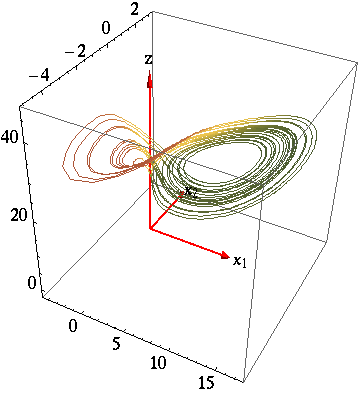
\includegraphics[width=0.40\textwidth]{CLEpcSect}
(b) %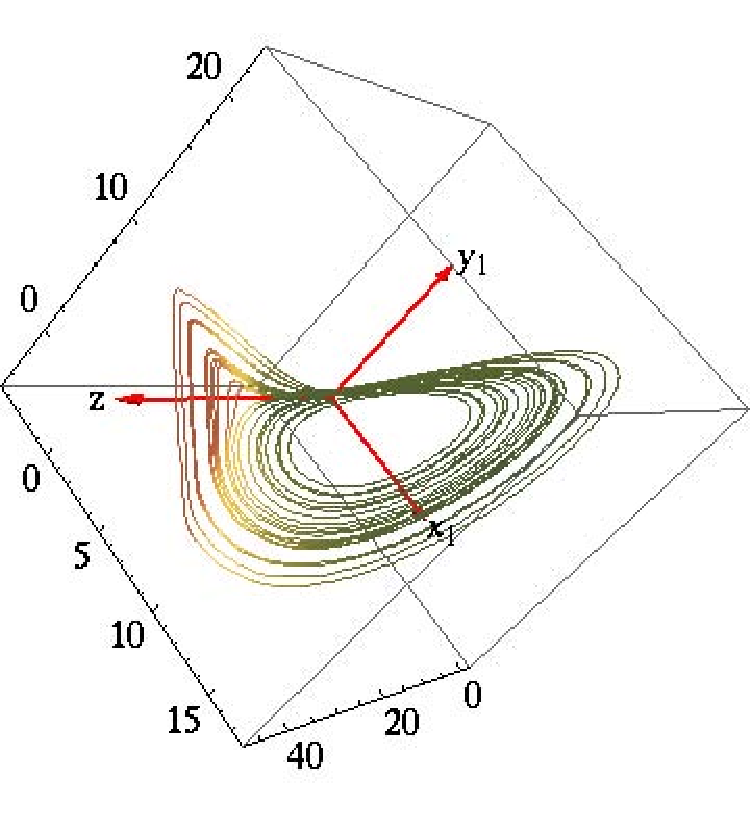
\includegraphics[width=0.43\textwidth]{CLEpcSect2}
\end{center}
\caption{
Method of moving frames, \slice\ fixed by a point on an
\reqv\ group orbit, $\sspRed = \ssp_{\REQB{}1}$. The strange
attractor of \reffig{fig:CLEx1x2z} in the \reducedsp\
of \refeq{EqMotionMovFramePC}:
(a) $\{x_1,x_2,z\}$ projection,
(b) $\{x_1,y_1,z\}$ projection.
Color-coding indicates $(\hat{\ssp} \cdot \hat{\sspRed})_4$
where $\hat{.}$ stands for unit vector, with green indicating values
of the inner product close to $1$ and brown indicating values
close to $0$.
    }
\label{fig:CLEpcSect}
\end{figure}
%%%%%%%%%%%%%%%%%%%%%%%%%%%%%%%%%%%%%%%%%%%%%%%%%%%%%%%%%%%%%%%%
%
A long time trajectory of \refeq{EqMotionMovFramePC} with
$x^*$ on the \reqv\ \REQB{1} group orbit is shown in
\reffig{fig:CLEpcSect}.
                                                        \exerbox{exer:PCsectionCLe}
    \PC{draw your own \reffig{fig:CLEpcSect}:\\
        * Mark $\ssp_{\REQB{}1}$ \\
        * Draw stable eigenvector of $\ssp_{\REQB{}1}$\\
        * State value of $\ssp_{\REQB{}1}$ somewhere
        }


%%%%%%%%%%%%%%%%%%%%%%%%%%%%%%%%%%%%%%%%%%%%%%%%%%
% computed by PCunrot.nb
\SFIG{ProblemsPill} %PCunrot1}
{}{
Method of moving frames, continuous time version, for the
$\slicep=(0,1,0,0)$,
$x_1=0,\;x_2>0$, \slice. The strange attractor of
\reffig{fig:CLEx1x2z} in the \reducedsp,
$\{x_2,y_2,z\}$ projection exhibits a discontinuity at
$x_2=0$.
}
{fig:PCunrot1}
%%%%%%%%%%%%%%%%%%%%%%%%%%%%%%%%%%%%%%%%%%%%%%%%%%

The method encounters singularities in
subsets of \statesp\rf{SiminosThesis}.
                                                    \exerbox{exer:csectionCLe}
A typical trajectory is shown in \reffig{fig:PCunrot1}.

\subsection{Integration on the \slice}

Our second method of symmetry reduction Siminos
\rf{SiminosThesis} calls {\em integration on the
\slice\ (II)}.

\fi
	
	
\section{\Slice\ singularities}
\label{sect:sliceSing}

Looking back at equation \refeq{eq:so2reduced}, we see that the \mslices\ potentially introduces singularities to the flow. When $\dotProd{\groupTan(\sspRed)}{\sliceTan{}}$ is zero, $\dot{\gSpace(\tau)}$ is not defined and as a consequence neither is the velocity in the slice. These singularities do not exist in the full space and are entirely artifacts of the \mslices. When the full space trajectory passes through one of these points the trajectory just passes through unhindered. The hope is then that these singularities do not greatly affect the trajectory in the reduced space.

	\ifarticle
	\else
	
In \refsect{sect:slices} we noted that the projection $f(\gSpace)$
can have inflection points,
    \PC{Are we only interested in Laplace-Beltrami operator on the
    group manifold
    \\
    \(
    \frac{\partial^2 ~~}{\partial \gSpace^2} f(\gSpace) =
    - \dotProd{\groupTan(\sspRed)}{\sliceTan{}} =
    \dotProd{\sspRed}{\dual{\Lg} \cdot {\Lg}\,\slicep}
    \)
    }
\beq
\frac{\partial^2 f(\gSpace_E)}
     {\partial \gSpace_a \partial \gSpace_b}
    =
  - \dotProd{\Lg_a e^{\gSpace_E \cdot \Lg} \ssp}{\sliceTan{b}}=
  - \dotProd{\groupTan_a(\sspRed_E)}{\sliceTan{b}}=0
\ee{PCinflPoint}
What role do they play? They are non-generic, but
if we consider projections of a successive instants of a trajectory
$f(\gSpace)=\dotProd{e^{\gSpace(t) \cdot \Lg} \ssp(t)}{\slicep}$, coalescence of
nearby minima, maxima pairs cannot be avoided. At the instant of coalescence
the denominator in \refeq{SF:sliceEas} goes through a simple pole,
and the integrated trajectory within slice jumps. Our next task is
to compute the size of the jump.
    \PC{`` from the principal value of the integrated velocity field on a trajectory through this singularity.'' Stefan, take it from here.}
    \PC{could it be that inflections are generic only for \SOn{2},
        but of higher codimension and thus not encountered
        by 1$d$ time trajectory for higher-dimensional Lie groups?}

Once we determine the trajectory point at which
a singularity occurs, we have to describe what happens to the \reducedsp\ trajectory when it passes through the singularity. The trajectory in the \reducedsp\ is given by $\sspRed(\tau)=\LieEl^{-1}(\tau) \ssp(\tau)$, so if we know how $\LieEl(\tau)=\exp({-\gSpace(\tau) \cdot \Lg})$ behaves as the trajectory passes through a singularity, then we know how the \reducedsp\ trajectory behaves.



\subsection{\CLe\ singularities}
\label{sect:cLeSing}

To answer this question, let us first look at the example of the \cLe. There is only one infinitesimal generator for the \SOn{2} symmetry group, so the rotation angle $\gSpace$ into the \reducedsp\ trajectory is given by \refeq{SL:CLEsliceRot}.

If $\ssp(\tau)$ is a trajectory in full state space, then the
 \reducedsp\ flow $\sspRed(\tau)$ goes through a singularity when
 $\dotProd{\groupTan_{}(\sspRed^*)}{\sliceTan{}}=0$
at time $\tau=0$, $\sspRed^* = \sspRed(0)$.
The angle $\gSpace^*$ for rotating a point into the slice must satisfy
    \PC{Isn't some of this already worked out in \refexam{exam:CLErotAngle}?
        You should refer to already derived results, rather than repeating
        the same text}
\bea
0             &=&
\dotProd{\ssp}{\sliceTan{}}\cos(\gSpace^*) +
\dotProd{\groupTan_{}(\ssp)}{\sliceTan{}}\sin(\gSpace^*)
    \continue
\tan(\gSpace^*) &=&
-{\dotProd{\ssp}{\sliceTan{}}}/{\dotProd{\groupTan_{}(\ssp)}{\sliceTan{}}}
 \,.
\label{SF:SO2angleRot}
% \refeq{SF:SO2angleRot}
\eea
This equation has two solutions
$\{\sspRed^*=\LieEl(\gSpace^*)\ssp, \LieEl(\gSpace^*+\pi)\ssp\}$
unless both $\dotProd{\sspRed^*}{\sliceTan{}}$
and $\dotProd{\groupTan_{}(\sspRed^*)}{\sliceTan{}}$ are zero,
in which case any angle works (this is exactly the situation
the trajectory is in when it passes through a singularity
$\ssp^*$).

Consider $\gSpace(\tau)$ approaching the singularity value
$\gSpace^*$ as $\tau \rightarrow 0$.
The trajectory is smooth, so it can be approximated by the linear
term in the Taylor expansion,
$
\ssp(\tau)=\sspRed^*+\vel^*\tau+O(\tau^2)
\,,\qquad
\vel^* = \vel(\sspRed^*)
    \,.
$
    \PC{Stefan had ``
$\ssp(\tau)=\ssp(0)+\vel(0)\tau+\Mvar(\tau^*)\frac{\tau^2}{2}$ where $\Mvar$ is the stability matrix and $\tau^*$ is between $0$ and $\tau$.
    '' This looks wrong to me. In any case, the oredr ${\tau^2}{2}$ term is
    not used.
% -\frac{\dotProd{\ssp(0)+\vel(0)\tau
% +\Mvar(\tau^*)\frac{\tau^2}{2}}{\sliceTan{a}}}{
% \dotProd{\Lg(\ssp(0)+\vel(0)\tau+\Mvar(\tau^*)\frac{\tau^2}{2})}{\sliceTan{}}}
    }
Hence as $\tau \rightarrow 0$,
\bea
\tan(\gSpace)
% = -\frac{\dotProd{\ssp}{\sliceTan{}}}{\dotProd{\groupTan_{}(\ssp)}{\sliceTan{}}}
&\rightarrow&
-\frac{\dotProd{\sspRed^*+\vel^*\tau}{\sliceTan{}}}
{\dotProd{\Lg(\sspRed^*+\vel^*\tau)}{\sliceTan{}}}
    \continue
\tan(\gSpace^*) &=&
     -\frac{\dotProd{\vel^*}{\sliceTan{}}}
      {\dotProd{\groupTan_{}(\vel^*)}{\sliceTan{}}}
\,.
\label{SF:snglrAngl}
\eea
So at the singular point the slice-rotation angle $\gSpace^*$ is computed as in
\refeq{SF:SO2angleRot}, but using $\vel^*$ rather than $\ssp^*$; as
$\ssp$ and  $\vel(\ssp)$ rotate rigidly together, that is OK.

If we add on the restriction $\dotProd{\groupTan_{}(\ssp)}{\sliceTan{}}$ \ref{def:movingFrame} be nonnegative so that we get a unique representative from each trajectory, then as the trajectory approaches the singularity $\dotProd{\groupTan_{}(\ssp)}{\sliceTan{}}\approx \tau \dotProd{\Lg\vel^*}{\sliceTan{}}$. As $\tau$ goes from negative to positive, this expression changes sign, so when the trajectory goes through the slice,
according to \refdef{def:movingFrame} we must rotate the trajectory by $\pi$ in order for it to satisfy the restriction.


    \fi

\subsection{Passing through a singularity}
\label{sect:passingSing}

The behavior of the \reducedsp\ trajectory is entirely determined by the $\gSpace$ used to rotate the full space trajectory into the slice. If we can find an expression for $\gSpace$ as the trajectory approaches a singularity then we know the behavior of the \reducedsp\ trajectory as it approaches a singularity.

Suppose the trajectory passes through a singularity at time $\tau=\tau_0$.
$\ssp(\tau)$ is $C^{\infty}$ since we can explicitly calculate any order derivative using $\dot{\ssp}=\vel(\ssp)$. This allows us to use Taylor expansions to approximate the trajectory at any time $\tau_0$; $\ssp(\tau)=\ssp(\tau_0)+\vel(\ssp(\tau_0)) (\tau-\tau_0)+O((\tau-\tau_0)^2)$. Being in the linear slice imposes the condition \refeq{PCsectQ1} on $\gSpace(\tau)$ for each infinitesimal generator $\sliceTan{a}$ of the Lie group at $\slicep$. Using the results of \refsect{sect:slices} we can rotate the trajectory in the full state space so that $\ssp(\tau_0)$ is in the slice and the equivariance of the flow \refeq{eq:FiniteRot} allows us to work with this equivalent trajectory. This gives us the restriction for $\gSpace$ in terms of the Taylor expansion:
\[
\dotProd{e^{\gSpace \cdot \Lg}(\ssp(\tau_0)+\vel(\ssp(\tau_0)) (\tau-\tau_0)+O(\tau^2))}{\sliceTan{a}}
\]
If in addition we know that all the higher order terms in the inner product are negligible compared to the linear term near $\tau_0$:
\beq
\dotProd{e^{\gSpace \cdot \Lg} O((\tau-\tau_0)^2)}{\sliceTan{a}}<<\dotProd{e^{\gSpace \cdot \Lg}\vel(\ssp(\tau))(\tau-\tau_0)}{\sliceTan{a}}
\ee{eq:neglig}
then we can take the limit of this expression as $\tau \rightarrow \tau_0$:
\bea
&&\dotProd{e^{\gSpace \cdot \Lg}(\ssp(\tau_0)+\vel(\ssp(\tau_0)) (\tau-\tau_0)+O(\tau^2))}{\sliceTan{a}}
    \continue
&\approx& \dotProd{e^{\gSpace \cdot \Lg}\ssp(\tau_0)+ e^{\gSpace \cdot \Lg}\vel(\ssp(\tau_0)) (\tau-\tau_0)}{\sliceTan{a}}
    \continue
&\approx&  \dotProd{e^{\gSpace \cdot \Lg}\vel(\ssp(\tau_0)) (\tau-\tau_0)}{\sliceTan{a}}
    \continue
&\approx&  (\tau-\tau_0)\dotProd{e^{\gSpace \cdot \Lg}\vel(\ssp(\tau_0))}{\sliceTan{a}}\approx 0
\,.
\eea
$\gSpace$ approaches $\gSpace^*$ such that $\dotProd{e^{\gSpace^* \cdot \Lg}\vel(\ssp(\tau_0))}{\groupTan(\slicep)}\approx 0$ so $\gSpace$ approaches an angle that rotates $\vel(\ssp(\tau_0))$ into the slice. Which angle it approaches before and after the singularity depend on the restrictions \ref{def:movingFrame} put on the slice, and the trajectory can jump from one $\gSpace$ to another depending on this choice. The only affect passing through a singularity will have on the \reducedsp\ trajectory then is to cause it jump from one point on a group orbit to another at the singularity, and the trajectory will be smooth otherwise.

\example{\CLe\ singularities.}
{
Suppose the singularity occurs at $\tau=0$. From \refexam{exam:CLErotAngle} we have the equation for $\gSpace$
\bea
\tan(\gSpace) &=&
\frac{-{\dotProd{\ssp}{\sliceTan{}}}}{{\dotProd{\groupTan_{}(\ssp)}{\sliceTan{}}}}.
\eea
Using the Taylor expansion for the trajectory and letting $\tau \rightarrow 0$ we find that:
\bea
\tan(\gSpace)
&=& -\frac{\dotProd{\ssp_0+\vel(\ssp_0)\tau+O(\tau^2)}{\sliceTan{}}}{\dotProd{\groupTan(\ssp_0+\vel(\ssp_0)\tau+O(\tau^2))}{\sliceTan{}}}
\continue
\tan(\gSpace)
&\rightarrow& -\frac{\dotProd{\ssp_0}{\sliceTan{}}+\tau\dotProd{\vel(\ssp_0)}{\sliceTan{}}+O(\tau^2)}{\dotProd{\groupTan(\ssp_0)}{\sliceTan{}}+\tau
\dotProd{\vel(\ssp_0)}{\sliceTan{}}+O(\tau^2)}
\continue
\tan(\gSpace) &\rightarrow&
     -\frac{\dotProd{\vel(\ssp_0)}{\sliceTan{}}}
      {\dotProd{\groupTan_{}(\vel(\ssp_0))}{\sliceTan{}}}
\,.
\label{SF:snglrAngl}
\eea
As predicted, $\gSpace$ approaches an angle that rotates $\vel(\ssp_0)$ into the slice.
Next add on the restriction $\dotProd{\groupTan_{}(\ssp)}{\sliceTan{}}$ \ref{def:movingFrame} be nonnegative, then as the trajectory approaches the singularity $\dotProd{\groupTan(\ssp)}{\sliceTan{}}\approx \tau \dotProd{\Lg\vel^*}{\sliceTan{}}$. As $\tau$ goes from negative to positive, this expression changes sign. Hence we must rotate the trajectory by $\pi$ to satisfy the condition.
}
%\SFIG{jump}
%{}{
%A $\{y_2,y_1,z\}$ plot of the \reducedsp\ \cLe\ trajectory with initial point passing $(x_1, x_2, y_1, y_2, z) = (1, 2, 3, 1, 2)$ through a singularity at time $\tau=0.1$ in the slice normal to $\sliceTan{}={-0.0345614, 0.16259, 0.0144152, -0.0789286, 0}$. The blue portion is the trajectory before the singularity, the purple and the yellow trajectories are the two possible continuations of the trajectory after the singularity (notice they differ by a rotation of $\pi$). The yellow trajectory is the one chosen by the constriant [ref]

%    }{fig:jump}

\example{$\SOn{2}$ singularities.}
{\label{ex:so2singularities}
Consider now the general from of an $\SOn{2}$ symmetry from \refexam{exam:SO2irrepst}. Plugging this into the slice condition \refeq{PCsectQ1} we find that
\bea
\dotProd{e^{\gSpace \Lg}\ssp}{\groupTan(\slicep)}=\dotProd{\ssp}{(\sum\limits_m (\cos(-m\gSpace) \id^{(m)}+\sin(-m\gSpace) \frac{1}{m}\Lg^{(m)})) \sliceTan{}}
\continue
=\sum\limits_m(\cos(m\gSpace) \dotProd{\ssp}{\Lg^{(m)} \slicep}-\sin(m\gSpace) \dotProd{\ssp}{\id^{(m)} \slicep})
\label{eq:so2sing}
\eea
Both $\cos(m\gSpace)$ and $\sin(m\gSpace)$ are expressible as polynomials of degree m in $\sin(\gSpace)$ and $\cos(\gSpace)$, so \refeq{eq:so2sing} is expressible of a polynomial whose coefficients are determined by $\dotProd{\ssp}{\Lg^{(m)} \slicep}$ and $\dotProd{\ssp}{\id^{(m)}}$. $\gSpace$ corresponds to a root of this polynomial. The coefficients of the polynomial vary smoothly with $\ssp$, so its roots vary smoothly too. This means \refeq{eq:neglig} is satisfied for these $\SOn{2}$ symmetries and we can use the result of \refeq{SF:snglrAngl}.
}

\subsection{Singularities of $\SOn{2} \times \SOn{2}$}

While most systems in fluid dynamics do not exhibit a single $\SOn{2}$ symmetry, many do have continuous symmetries which are the products of $\SOn{2}$ groups, each of which act on different coordinates of the state space. The \KS\ equations \rf{ku,siv}, plane-couette flow \rf{Visw07b,GHCW07,HGC08,HalcrowThesis}, and pipe flow \rf{Wk04,Kerswell05} all have continuous symmetries of this form.

                                                    %\toCB
% PC cribbed from Penrose p. 254:
\begin{definition}
\label{def:productGroup}
\textbf{Product group.}
If \Group\ and H are any two groups, than they can be combined in
what is called the {\em product group} $\Group \times H$, whose
elements are pairs $(\LieEl,h)$, where $\LieEl$ belongs to \Group, and
$h$ belongs to $H$, with the group multiplication rule
\[
(\LieEl_1,h_1)(\LieEl_2,h_2)=(\LieEl_1 \LieEl_2,h_1 h_2)
\,.
\]
\end{definition}

Suppose that the state space is the product of two spaces, $\mathbb{X}=\mathbb{A} \times \mathbb{B}$.
Let $\Group$ be a Lie group with two infinitesimal generators, $\Lg_1$ and $\Lg_2$, such that the $e^{\gSpace_1 \Lg_1}$ action on $\mathbb{X}$ fixes the $\mathbb{B}$ coordinates ($e^{\gSpace_1 \Lg_1} \, (a,b)=(a',b')$ where $b'=b$) and $e^{\gSpace_2 \Lg_2}$ fixes the $\mathbb{A}$ coordinates ($\Group$ is the direct product of two $\SOn{2}$ groups which act on different coordinates of $\mathbb{X}$).

We begin by looking at the action of infinitesimal rotations of $\Lg_1$. $e^{\delta \gSpace_1 \Lg_1}(a,b)=(1+\delta \gSpace_1 \Lg_1) (a,b)$\refeq{eq:infinitesimal}. $e^{\delta \gSpace \Lg_1}$ fixes the $\mathbb{B}$ coordinates, so $e^{\delta \gSpace \Lg_1}=(a',b)$ for some $a'$. This results in $(a',b)=(a,b)+\delta \gSpace_1 \Lg_1(a,b)$ so $\delta \gSpace_1 \Lg_1(a,b)=(a'-a,0)$. This is true for any $\delta \gSpace_1$, so $\Lg_1$ maps the $\mathbb{B}$ coordinates to 0. The same argument gives us that $\Lg_2$ maps the $\mathbb{A}$ coordinates to 0. Looking at $\Lg_1 \Lg_2$ we find $\Lg_1 \Lg_2 (a,b)=\Lg_1 (0,b')=(0,0)$ for any $(a,b) \in \mathbb{X}$, which is only possible if $\Lg_1 \Lg_2=0$. The same argument tells us that $\Lg_2 \Lg_1=0$ %(this also follows from $\Lg_1 \Lg_2=0$ and the fact that the $\Lg_i$ are antihermitian).

We can now use $\Lg_1 \Lg_2=\Lg_2 \Lg_1=0$ to demonstrate a significant result about the singularities of this symmetry group.

Suppose we are rotating a trajectory $\ssp(\tau)$ into the slice normal to the group tangents at $\slicep$. Using $\sliceTan{a}=\groupTan_1(\slicep)$ for equation \refeq{eq:slicecondition} tells us that
$\dotProd{\vel(\sspRed)}{\groupTan_1(\slicep)}-\dot{\gSpace_1} \dotProd{ \groupTan_1(\sspRed)}{\groupTan_1(\slicep)}-\dot{\gSpace_2} \dotProd{ \groupTan_2(\sspRed)}{\groupTan_1(\slicep)}=0$.

We have
$\dotProd{\groupTan_2(\sspRed)}{\groupTan_1(\slicep)}=0$ since $\Lg_1 \Lg_2=0$,
leaving us with $\dotProd{\vel(\sspRed)}{\groupTan_1(\slicep)}-\dot{\gSpace_1}\dotProd{\groupTan_1(\sspRed)}{\groupTan_1(\slicep)}=0$. This gives us the equation for $\dot{\gSpace_1}$:
\beq
\dot{\gSpace_1}=\frac{\dotProd{\vel(\sspRed)}{\groupTan_1(\slicep)}}{\dotProd{\groupTan_1(\sspRed)}{\groupTan_1(\slicep)}}
\eeq
This is the same as equation \refeq{eq:so2reduced} for the rotation group consisting of only the rotations generated by $\Lg_1$. This equation is independent of the action of $\Lg_2$. This means a point being singular depends only on whether or not it is singular in either of the slices normal to only one of the group tangents. This permits us to break up the problem of determining if a point is singular and how this affects the \reducedsp\ trajectory for the entire group into the same problem for each of the $\SOn{2}$ groups generated by one of the infinitesimal generators, a situation we are comfortable with.

This makes sense since if a point $\sspRed$ is in the slice normal to $\groupTan_2(\slicep)$ then any point in the $\Lg_1$ orbit is in the slice since $\dotProd{e^{\gSpace_1 \Lg_1}\sspRed}{\groupTan_2(\slicep)}=\dotProd{(1+\gSpace_1 \Lg_1+\ldots)\sspRed}{\groupTan_2(\slicep)}=\dotProd{\sspRed}{\groupTan_2(\slicep)}+\dotProd{\gSpace_1 \Lg_1 \sspRed}{\groupTan_2(\slicep)}+\ldots=0$. The first inner product is zero because we assumed that $\sspRed$ was in the slice and the rest of terms are zero because $\Lg_1 \Lg_2=0$. So the only restriction for the values of $\gSpace_1$ that rotate the point into the slice are the restrictions it gets from the $\groupTan_1(\slicep)$ condition.

This argument is easily extended to a product of arbitrarily many $\SOn{2}$ acting on different coordinates of the state space (any two of the $\SOn{2}$ act on distinct coordinates so the singularities are pairwise independent).
In \refexam{ex:so2singularities} we found a simple description for what happens to the \reducedsp\ traectory as it passes through singularity of a single $\SOn{2}$ symmetry group (it is rotated by a finited amount), so using this result, we can handle the singularities for the product of arbitrarily many $\SOn{2}$ groups which pairwise act on different coordinates of the state space.


    \ifarticle
    \else

\subsection{\Reqva\ stability in a linear slice}

As an example of this we will calculate the stability matrix of a relative equilibrium ([refedef]) in a slice.

%\[
%\MvarRed_{ij} =
%\Mvar_{ij}-c I_{ij} -(\groupTan(\ssp))_i\,(\frac{\dotProd{\frac{\partial v}{\partial x_i}}{\sliceTan{}}}
%        {\dotProd{\groupTan(\ssp) { \sliceTan{}}}}
%      - c \frac{\frac{\partial (Tx)}{\partial x_j}\cdot \sliceTan{}}{Tx \cdot \sliceTan{}})
%\]

\beq
{\MvarRed}(\sspRed)_{ij} = \Mvar(\sspRed)_{ij}-\velRel \cdot \Lg_{ij}
     -\groupTan(\sspRed)_i\,\left(
     \frac{\frac{\partial v}
     {\partial x_j}\cdot \groupTan(\sspRed)}{\dotProd{\groupTan(\sspRed)}{\sliceTan{}}}
     - \velRel \frac{\frac{\partial (\groupTan(\sspRed))}
              {\partial x_j}\cdot \sliceTan{}
              }{\dotProd{\groupTan(\sspRed)}{\sliceTan{}}}
              \right)
\ee{SF:redJacob1}



\section{Relative stability}
\label{sect:relStab}
%\PC{Write up here stability of relative solutions following \refref{DasBuch},
%\\
%\wwwcb{/chapters/continuous.pdf}
%    }


\subsection{\Reqva}

A \reqv\ is a trajectory that stays
within a group orbit of the symmetry group.

For a \reqv\ \REQV{}{} the flow and the group tangent vectors coincide, and
any point on the \reqv\ orbit is a fixed point in the co-moving frame,
a frame moving with velocity
    %\toCB
\beq
\vel(\ssp) - \velRel \cdot \groupTan(\ssp) =0
    \,,\qquad
\ssp \in \pS_{\REQV{}{}}
\,.
\ee{SF:reqvTangent}
Dotting
$
\groupTan_a(\vel)  - \Mvar(\ssp) \, \groupTan_a(\ssp) =0
$,
the
equivariance condition \refeq{eq:InfnmslRot}, by the velocity $c$,
I get
\beq
( \Mvar -  \velRel \cdot \Lg) \vel =0
\,.
\ee{ReqvMargEig}
In other words, you have to be in the co-rotating
frame for eigenvalue to be marginal, and the velocity
be the corresponding right eigenvector.

In order for a trajectory to stay in the group orbit, its
velocity must always point in the tangent direction to the
group action, so we must have $\vel(\ssp) = \velRel(\tau)
\cdot \groupTan(\ssp)$ where $\velRel(\tau)_a$ is a scalar
function in terms of time.
    \PC{scalar? $\velRel(\tau)_a$ is an $N$-dimensional vector for
    $N$-dimensional group $\Group$. You are showing that
    for a compact Lie group $\velRel(\tau)_a = \velRel_a$ is constant
    independent of time, but the proof feels a bit clumsy.}
We also know that $x(\tau) = \LieEl(\tau) x(0)$ for some
element $\LieEl(\tau)$ of the symmetry group. Inserting this
into the first equation, we get that
\bea
\vel(\LieEl(\tau) \xInit) &=&
    \velRel(\tau)\cdot \groupTan(\LieEl(\tau) \xInit)
    \continue
\LieEl(\tau) \vel(\xInit) &=&
    \LieEl(\tau) \, \velRel(\tau) \cdot \groupTan(\xInit)
    \continue
\vel(\xInit) &=& \velRel(\tau) \cdot \groupTan(\xInit)
\eea
both $\vel(\xInit)$ and $\groupTan(\xInit)$ are independent
of time, and we have $\velRel(\tau) = \velRel(0) = \velRel$
for all $\tau$, so $\velRel$ is constant. If \SOn{n} is a
rotational symmetry, $\velRel$ is called the `angular'
velocity of the {\reqv}.

To further visualize the drifting of the flow around the
$z$-axis, we next find and plot the relative equilibria of
the \cLe. A {\reqv} is a solution of the flow which appears
stationary in a frame rotating at the appropriately chosen
constant angular velocity. We find these points in a manner
similar to finding the equilibria, with one difference. As
the flow drifts (rotates), a {\reqv} will drift as well, so
that instead of setting all of the $\vel(x)=0$, we allow the
component of $\vel(x)$ tangent to direction of group rotation to
be non-zero.

\subsection{Computing and plotting the {\reqv} $\REQB{1}$}

%                                              \exerbox{exer:CompRelEqu}
%                                              \exerbox{exer:PlotPolEqu}

Rebecca got for
$\REQB{1}$ in Cartesian coordinates
%                                             \exerbox{exer:PlotRelEqu}
\[\ssp_{\REQB{}1} = (8.48492,0.0771356,8.48562,0,26.9999)
\,,
\]
but I get (???).
\refFig{fig:CLERelEqui} shows the \cLf\ with initial point at
$\ssp_{\REQB{}1}$. The {\reqv} begins by tracing out a circle
around the $z$-axis, showing how the flow drifts. Eventually
numerical errors accumulate and the circle turns into a
``horn'' shape when the flow begins to spiral out.
%%%%%%%%%%%%%%%%%%%%%%%%%%%%%%%%%%%%%%%%%%%%%%%%%%%%%%%
% computed in equilibrium.nb
\begin{figure}[h]
\begin{center}
(a) % ~\includegraphics[width=0.35\textwidth]{CLERelEqui}
(b) % ~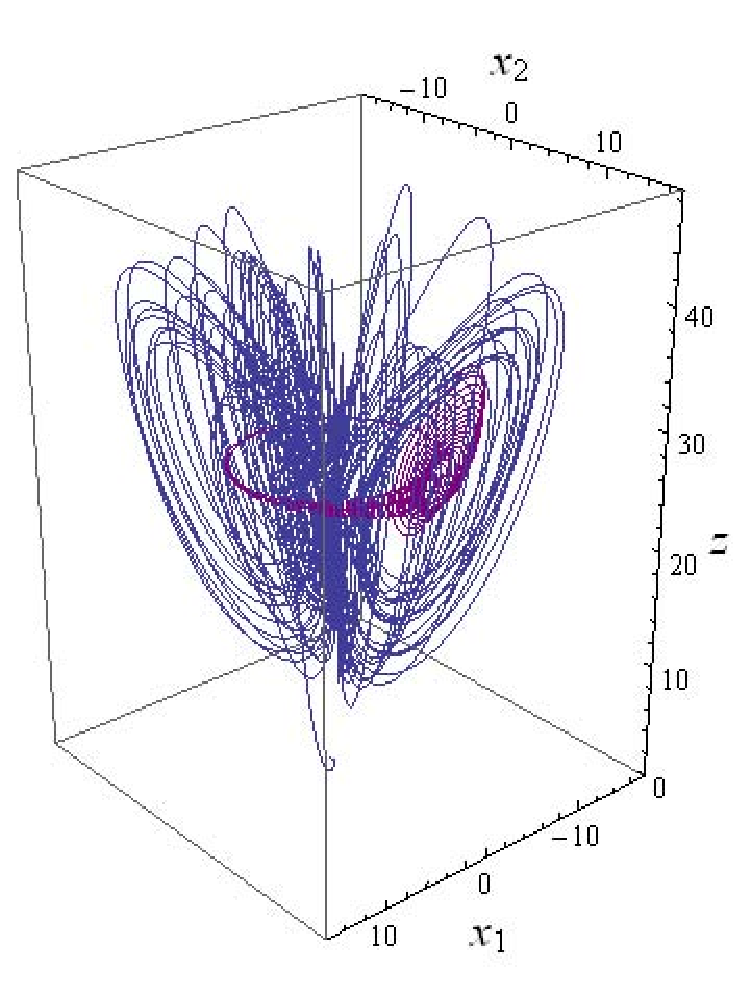
\includegraphics[width=0.35\textwidth]{CLEx1x2zRelEqu}
\end{center}
\caption{
Cartesian $\{x_1,x_2,z\}$ plot of the \cLf\ (a) with initial point
close to $\REQB{1}$, (b) superimposed over the strange attractor of
\reffig{fig:CLEx1x2z}.
    }
\label{fig:CLERelEqui}
\end{figure}
%%%%%%%%%%%%%%%%%%%%%%%%%%%%%%%%%%%%%%%%%%%%%%%%%%%%%%%

From
here on, we examine the properties of the point defined
above as $\ssp_{\REQB{}1}$.

\subsection{\Rpo s}
\label{SF:rpos}

\paragraph{Definition:
           \Rpo}
$p$ is an orbit $\pS_p$ in {\statesp} $\pS$, a set of relative periodic
points exactly recur
    %\toCB
\beq
\ssp (0) = \LieEl_p \ssp (\period{p} )
    \,,\qquad
\ssp (\tau) \in \pS_p
    \,,
\label{RPOrelper1}
\eeq
at a fixed {\em relative period} $\period{p}$, but
shifted by a fixed group action ${\LieEl_p}$
which brings the endpoint $\ssp (\period{p} ) $
back into the initial point $\ssp (0) $.
The group action ${\LieEl_p}=\LieEl(\gSpace_p)$ parameters  %\toCB
$\gSpace = (\gSpace_1,\gSpace_2,\cdots\gSpace_N)$
are referred to as ``phases,'' or ``shifts.''
%
In general these phase are irrational, and the trajectory  %\toCB
sweeps out ergodically the group orbit without ever closing
into a \po.

In presence of a continuous symmetry we define the
\emph{{\FloquetM} for a \rpo} as the {\jacobianM} evaluated
at the period $\period{p}$ and rotated back into a \po\ by the
group action $\LieEl(\gSpace_p)$:
    %\toCB
\beq
 \jMps_p(\ssp) = \LieEl(\gSpace_p)\jMps^\period{p}(\ssp)
    \,,\qquad
\ssp  \in \pS_p
\,.
\ee{SF:symPrimJac}
The argument of \refsect{sect:SFpos} goes through also in
the presence of a group rotation,
and \refeq{SF:transpEigPO} is correct for \rpo s as well.

\subsection{Marginal eigenvalues}

The {\jacobianM} of a periodic orbit has marginal eigenvalues
when there is either a continuous symmetry (which can use to
reduce the problem) or a non-hyperbolicity in the flow (which
is not as easy to deal with).

To see that each continuous symmetry has a corresponding
marginal eigendirection, let $\ssp$ be any point on a periodic
orbit p with period $\period{p}$. If $\LieEl$ is any element in
the continuous symmetry Lie group $\Group$, then $f^t(\LieEl \ssp)
= \LieEl f^t(\ssp)$. By definiton, $\jMps^t(\ssp)
\delta \ssp = \delta f^t(\ssp)$.
Close to identity $\LieEl = 1+\delta
\theta \cdot \Lg$ is an infinitesimal Lie group element and
$\delta \ssp = \ssp - \LieEl \ssp = \ssp - (1+\delta \theta
\cdot \Lg) \ssp  = \delta \theta \cdot \Lg \ssp,$
so
$\delta f^{\period{p}}(\ssp) = f^{\period{p}}(\ssp) -
f^{\period{p}}(\LieEl \ssp)= f^{\period{p}}(\ssp) - \LieEl f^{\period{p}}(\ssp) =
\ssp - \LieEl \ssp = \delta \theta \cdot \Lg \ssp$.
This gives us
$\jMps_p(\ssp) \delta \theta \cdot \Lg \ssp = \delta
\theta \cdot \Lg \ssp$,
\ie, a set of marginal direction eigenvectors
\beq
 \jMps_p(\ssp) \groupTan_{a}(\ssp) =
\groupTan_{a}(\ssp)
\ee{SF:symMargEig}
with unit eigenvalues $\ExpaEig_a=1$,
where $\groupTan_{a}(\ssp)$ is a group tangent \refeq{PC:groupTan}.
    \PC{prove this for a \rpo, using definition \refeq{SF:symPrimJac};
        the \po\ marginal eigenvalue should be a special case.}


\subsection{Stability of \reqva\ in \reducedsp}
%SF June 22 2010

Using the parameters \refeq{SiminosPrmts}, we get the
 $\REQB{1}$ stability eigenvalues
\[
0.0938 \pm 10.1945i,-22.0000,-13.8534,-11.009
\]
with corresponding eigenvectors
        \PC{ChaosBook convention is to order eigenvalues
        from most positive (unstable) to the most negative.
        \\
        Replace complex eigenvectors by the real,
        imaginary parts, as that is what you actually use - I
        did this in \refeq{eigVecQ1}.
        }
\bea
&&(0.3378\mp 0.3411i,0.6887,0.0017\mp 0.0031i,0.5133\mp 0.1706i,-0.0029\mp 0.0511i)
\continue
&&(0.9939,0.0470,0.0009,-0.0994,0.0051)
\continue
&&(-0.8966,0.3457,0.0097,-0.2755,0.0246)
\continue
&&(0.0210,-0.0203,-0.995,0.0095,-0.0011)
\nnu
\eea
These are the same as the eigenvalues found using polar coordinates with the addition of $-22.0000$.
    \PC{
    ``the addition of $-22.0000$'' means what?
    }

The equations of motion for trajectory kept in a hyperplane by rotation under the symmetry group are:
\bea
    \dot{\gSpace}_a (\sspRed) &=&
    \frac{\dotProd{\vel(\sspRed)}{\sliceTan{a}}}
         {\dotProd{\groupTan(\sspRed)}{\sliceTan{}}}
    \continue
    u(\sspRed) &=& \vel(\sspRed)-\dot{\gSpace}(\sspRed)  \cdot \groupTan(\sspRed)
\eea
where $\vel(\sspRed)$ is the velocity of the full \statesp\ flow, $\groupTan(\sspRed)$ is the tangent to the group action, and $\sliceTan{}$ is the vector normal to the hyperplane of the slice. Using this equation we get that the {\stabmat} $\MvarRed$ for the system in \reducedsp\ is given by:
    \PC{Stefan's version was
\[
M_{ij} =
A_{ij}-c I_{ij} -(Tx)_i\,(\frac{\frac{\partial v}{\partial x_i}\cdot \sliceTan{}}
        {Tx \cdot \sliceTan{}}
      - c \frac{\frac{\partial (Tx)}{\partial x_j}\cdot \sliceTan{}}{Tx \cdot \sliceTan{}})
\]
    hopefully no errors introduced in my rewrite
    }
\beq
{\MvarRed}(\sspRed)_{ij} = \Mvar(\sspRed)_{ij}-\velRel \cdot \Lg_{ij}
     -\groupTan(\sspRed)_i\,\left(
     \frac{\frac{\partial v}
     {\partial x_j}\cdot \sspRed}{\dotProd{\groupTan(\sspRed)}{\sliceTan{}}}
     - \velRel \frac{\frac{\partial (\groupTan(\sspRed))}
              {\partial x_j}\cdot \sliceTan{}
              }{\dotProd{\groupTan(\sspRed)}{\sliceTan{}}}
              \right)
\ee{SF:redJacob1}

                                                    \exerbox{exer:Reducedstab}

\subsection{Eigen-system of the slice \stabmat}

As in \refsect{sect:stability}, we now find and plot the
eigen-system of the \stabmat\ in order to understand the
stability of $\REQB{1}$.
Rebecca finds the eigenvalues
\beq
(\lambda_{1,2},\lambda_3,\lambda_4)
= (0.0938179 \pm 10.1945 i,-11.0009,-13.8534)
\ee{RW:REQB1eigvals}
with the eigenvectors
\bea
\Re e_{1} &=& \Re e_{2} = (-0.266121, -0.0321133, 0.00034139, 0.719222)
\continue
\Im e_{1}  &=& -\Im e_{2} = (-0.295017, 0.569063, -0.000551886,0)
\continue
e_3 &=& (-0.0883591, -0.0851485, -0.989135, -0.0809553)
\continue
e_4 &=& (-0.855586, -0.329912, -0.00273531, -0.398902)
\,.
\label{eigVecQ1}
\eea

As in \refsect{sect:stability}, we can also plot the flow
with an initial point very near to
$\REQB{1}$ along one of the eigenvectors.
% \refFig{fig:CLEQ1} shows just this.
                                                    \exerbox{exer:EigenQ1}
                                                    \exerbox{exer:PlotPolEigenQ1}

\subsection{\Rpo\ stability in \reducedsp}

    \PC{Stefan, please write up your ``three programs for approximating the \jacobianM\ along any trajectory.'' Derive here \rpo\ {\monodromyM} in the \reducedsp, test it on some of the Evangelos \rpo s for \cLe.
    }

\section{Newton searches for \po s}

We have already seen how knowing periodic orbits and their
stability can help us to understand the dynamics of the
system, but there still is the question of how to actually
find periodic orbits.

Suppose we are trying to find the periodic orbits of a
system. This means we want to find $x$ and $T$ such that $\ssp =
f^T\left(\ssp\right)$,
% $\Rightarrow 0 = \ssp-f^T\left(\ssp\right)$
where $f^T$ is the trajectory at
time $T$. We shall use Newton's method to search zeros of the function
$F\left(\ssp,T\right) = \ssp - f^T\left(\ssp\right)$. Let
$\left(\ssp,T\right)$ be an initial guess for Newton's method
close to an actual solution $\left(\ssp + \Delta x,T + \Delta
T\right)$, \ie\ $0 = \ssp +\Delta \ssp - f^{T+\Delta
T}\left(\ssp + \Delta \ssp\right)$. Keeping the Taylor series
to linear order
\[
0 \approx \ssp-
f^T\left(\ssp\right) + \left(I -
\jMps\left(\ssp\right)\right)\Delta \ssp -
v\left(f^T(\ssp)\right)\Delta T
\]
we get the Newton iteration estimate for
$(\Delta \ssp,\Delta T)$

We already know that if $\ssp$ is on a periodic orbit then
$
% \jMps\left(\ssp\right) \vel(\ssp) = v\left(\ssp\right) \Rightarrow
\left(I-\jMps\left(\ssp\right)\right) v\left(\ssp\right) =
0$, so $I-\jMps\left(\ssp\right)$ becomes
non-invertible as $\ssp$ approaches a periodic orbit.
%$\left(I-\jMps\left(\ssp\right)\right) v\left(\ssp\right)\approx 0$.
If $\Delta x$ is in the direction of
$v\left(\ssp\right)$ then
$\left(I-\jMps\left(\ssp\right)\right) \Delta \ssp \approx 0$
so the equation becomes very costly to solve accurately. This
means that we need to constrain the $\Delta \ssp$ to be
transverse to the flow during a Newton's iteration. We do this
by requiring $\Delta x$ satisfy
\beq
v (\ssp)^T \Delta \ssp = 0
\,.
\ee{SF:NewtonTransv}
We then get the system
\beq
    \begin{pmatrix}
        I-\jMps(\ssp)& \partial \vel(\ssp)\\
        \vel(\ssp)& 0
    \end{pmatrix}
    \begin{pmatrix}
        \Delta \ssp\\
        \Delta t
    \end{pmatrix}
    =-
    \begin{pmatrix}
        \ssp - f(\ssp)\\
        0
    \end{pmatrix}
\eeq
This problem was caused by the velocity vector being an
eigenvector of the {\jacobianM} with unit Floquet
multiplier. Thus for every unit Floquet multiplier we
need to add a constraint. It was
already shown that for every dimension of a continuous
symmetry there is a unit Floquet multiplier. For each of
these we need to add a constraint
similar to \refeq{SF:NewtonTransv}.

Next consider the same situation, but instead we will use a
cost (or error) function $I\left(\Delta \ssp\right) =
\left(\ssp + \Delta \ssp - f\left(\ssp + \Delta
\ssp\right)\right)^2/2$. If $\ssp+\Delta \ssp$ is on a
periodic orbit then $I\left(\delta \ssp\right)$ and its
linear in $\Delta x$ approximation  $\left(\ssp + \Delta \ssp
- f\left(\ssp+ \delta
\ssp\right)\right)\left(I-\jMps\left(\ssp\right)\right)$ are
both equal to 0. This cost function measures how
far the point $\ssp+ \Delta \ssp$ is from being a zero of the
function $F(\ssp, \Delta \ssp) = \ssp - f(\ssp)$. The cost
function gives a non-negative value, and its zeros are the
points on periodic orbits, so if we can find a way to
minimize the function then we would either find a periodic
orbit or learn that there are not any near our initial guess
(if the local minimum is not zero then there is no zero
nearby).

The linear approximation of the cost function is zero at a
periodic orbit, so the cost function is dominated by the
second order term near the orbits. Expanding $I(\Delta \ssp)$
to the second order, we get that $I \approx \tilde{\Delta
\ssp}^2/2 + (\ssp - f(\ssp)) \tilde{\Delta \ssp} +
(\ssp-f(\ssp))^2/2$ where $\tilde{\Delta \ssp} =
(I-\jMps(\ssp))\Delta \ssp$.
    \fi %end of article switch

\section{Constructing Invariants of the symmetry}

When dealing with a system with symmetry, knowing invariants of the symmetry group can be very useful \rf{OlverInv}. Reducing the symmetry using a slice provides a simple means of calculating invariants of a symmetry \rf{FelsOlver98,FelsOlver99}. The representatives in the slice are for entire group orbits, so if you find a formula for the representative in terms of the initial point, this equation is necessarily left invariant under the group action.
Ref. \rf{FelsOlver98,FelsOlver99} provide a detailed explaination of how this can be done efficiently for more general symmetry groups.

\example{Invariants for \cLe.}{
Consider the slice normal to the vector $(1,0,0,0,0)$ for the $\SOn{2}$ symmetry of the \cLe. Using equation \refeq{SL:CLEsliceRot} we find that a point $(x_1,x_2,y_1,y_2,z)$ will be rotated to the point
\begin{equation*}
(0,\, r_1,\, \frac{x_2 y_1 - x_1 y_2}{r_1},\, \frac{x_1 y_1 + x_2 y_2}{r_1},\, z)
\end{equation*}
where $r_1=\sqrt{x_1^2+x_2^2}$.
The equations for each of these coordinates are invariants of the flow. These differ only by a factor of $r_1$ from the Hilbert basis \refeq{eq:ipLaser} of \rf{SiminosThesis,DasBuch}.
}


	\ifarticle
	\else

\section{Hilbert polynomials}
\label{SF:relStab}

The polynomials \refeq{eq:ipLaser} form a Hilbert basis for the \cLe.
\beq
\begin{split}
    u_1 &= x_1^2+x_2^2 \cont
    u_2 &= y_1^2+y_2^2 \cont
    u_3 &= x_1 y_2-x_2 y_1\cont
    u_4 &= x_1 y_1+x_2 y_2\cont
    u_5 &= z\,.
    \label{eq:ipLaser}
\end{split}
\eeq
In terms of the polar coordinates for the \cLe, these polynomials are
	\PC{shouldn't the first two be $\rho_1^2,\rho_2^2 $?}
\beq
\begin{split}
    u_1 &= \rho_1 \cont
    u_2 &= \rho_2 \cont
    u_3 &= - \rho_1 \rho_2 \sin \theta \cont
    u_4 &= \rho_1 \rho_2 \cos \theta \cont
    u_5 &= z\,.
    \label{eq:hilPolar}
\end{split}
\eeq
The \cLe\ in the Hilbert basis are:
\beq
\begin{split}
  \dot{u}_1 &=2\,\sigma\,(u_4-u_1)\,,\\
  \dot{u}_2 &=-2(\,u_2 - r_2\, u_3 -\,(r_1-u_5)\,u_4)\,,\\
  \dot{u}_3 &=-(\sigma\, +1)\,u_3+r_2\, u_1+e\, u_4\,,\\
  \dot{u}_4 &=-(\sigma\, +1)\,u_4+\,(r_1-u_5)\,u_1+\sigma\, u_2-e\,u_3\,,\\
  \dot{u}_5 &=u_4-b\, u_5\,.
\end{split}
\label{eq:CLEip}
\eeq
The {\reqv} in polar coordinates is
\[
( \rho_1 , \rho_2 , \theta , z ) = (\sqrt{b (r_1 -d)},\sqrt{b d (r_1 -d)},\theta_Q, r_1 -d)
\]
where $d = 1+ \frac{e^2}{(\sigma +1 )^2}$ and $\theta_Q$ is the angle such that
\[
\cos \theta_Q = \sqrt \frac{1}{d}
    \,,\qquad
\sin \theta_Q = -\sqrt \frac{d-1}{d}
\,.
\]

\exercise{Hilbert basis singularities}{\label{exer:CLEipSyz}
% Predrag extracted from siminos/blog/CLEflotsam      Jun  5 2010
% also ChaosBook \example{Hilbert basis singularities}{\label{exam:CLEipSyz}
%
When one takes syzygies into account in rewriting a
dynamical system, singularities are introduced. For instance,
eliminate $u_2$ using the syzygy, and show that you get
the reduced set of equations,
	\PC{I removed
$  \dot{u}_2 = -2\left(\,\frac{u_3^2+u_4^2}{u_1} - \rho_2\, u_3
                -\,(\rho_1-u_5)\,u_4\right)
$
            }
\bea
  \dot{u}_1 &=& 2\,\sigma\,(u_4-u_1)
                \continue
  \dot{u}_3 &=& -(\sigma\, +1)\,u_3+\rho_2\, u_1+e\, u_4
                \continue
  \dot{u}_4 &=& -(\sigma\, +1)\,u_4+\,(\rho_1-u_5)\,u_1
                +\sigma\, {(u_3^2+u_4^2)}/{u_1}-e\,u_3
                \continue
  \dot{u}_5 &=& u_4-b\, u_5
\,,
\label{eq:CLEipSyz}
\eea
singular as $u_1\rightarrow 0$. (PC: check this - there might
be errors)
\authorES{}
    } %end \exer{Hilbert basis singularities}

The {\stabmat} in the Hilbert basis for the \cLe\ is
	\PC{This is [5$\times$5], but there are only 4 independent
            variables. How does that show up in the eigensystem of
	    {\stabmat}?}
\beq
\begin{split}
\mathbb{A}=
\left(
\begin{array}{ccccc}
-2 \sigma & 0 & 0 & 2 \sigma & 0\\
0 & -2 & 2 r_2 & 2 (r_1 - u_5) & -2 u_4\\
r_2 & 0 & -(\sigma +1 ) & e & 0\\
(r_1 -u_5 ) & \sigma & -e & -(\sigma +1 ) & -u_1\\
0 & 0 & 0 & 1 & -b
\end{array}
\right)
\end{split}
\eeq

\section{Raw \slice s}
\label{sect:raw}
    \PC{this is temporary, until \refsect{sect:slices} is finalized.
        Stefan, please compare the formulas in the two, in order to
        improve your \LaTeX\ arts, then remove this section.}

Our goal is to show that if we choose the slice to be the hyperplane normal to the group tangents at a point, then this slice intersects all group orbits.

For this proof we will assume that the Lie group is compact and connected (so we can represent any group element by $\LieEl=e^{\gSpace \cdot \Lg}$ where $\gSpace \cdot \Lg=\sum \gSpace_a \Lg_a$).\\
\\
\noindent Fix $\slicep \in \pS$.\\
We will be looking at the hyperplane $\bar{\pS}$ that is normal to all the group rotation tangents at $\slicep$, \ie\ all points $\ssp$ with $<\ssp|\groupTan_a(\slicep)>=0$ (where $\groupTan_a(\slicep)=\Lg_a \slicep$ are the group tangents at $\slicep$).\\
\\
Let $\ssp \in \pS$ be any point in the phase space.\\
We want to show that there is a point on the group orbit of $\ssp$ which lies in $\bar{\pS}$, \ie\ there is a group element $\LieEl=e^{\gSpace \cdot \Lg}$ such that $<\LieEl \ssp|\groupTan_a(\slicep)>=0$ for all $a$.\\
\\
To show this we will look at the function $f_{\ssp}(\gSpace)=<\slicep|e^{\gSpace \cdot \Lg} \ssp>$.\\
$f_{\ssp}$ is a continuous and differentiable function by how it was defined ($e^{\gSpace \cdot \Lg}$ is both continuous and differentiable and $f_{\ssp}$ is just the inner product of this with a constant, so it is also continuous and differentiable).\\
This tells us that if $\gSpace_E$ is an extremum of $f_{\ssp}$ then all of the first order partial derivatives of $f_{\ssp}$ will be zero at $\gSpace_E$ since $f_{\ssp}$ is differentiable.\\
This would mean $\frac{\partial f_{\ssp}(\gSpace_E)}{\partial \gSpace_a}=0$, so $<\slicep|\Lg_a e^{\gSpace_E \cdot \Lg} \ssp>=0$.\\
$\Lg_a$ is anti-hermitian, so $0=<\slicep|\Lg_a e^{\gSpace_E \cdot \Lg} \ssp>=<-\Lg_a \slicep|e^{\gSpace_E \cdot \Lg} \ssp>=-<\Lg_a \slicep|e^{\gSpace_E \cdot \Lg} \ssp>$ giving us that $<\groupTan_a(\slicep)|e^{\gSpace_E \cdot \Lg} \ssp>=0$.\\
We therefore have that $e^{\gSpace_E \cdot \Lg} \ssp$ is normal to all the group tangents of $\ssp$ so it is in $\bar{\pS}$.\\
This means that any extrema of $f_{\ssp}$ are in the slice.\\
All that is left to do then is to show that $f_{\ssp}$ has extrema.\\
\\
Define $h(y)=<\slicep|y>$.\\
$h$ is continuous it is the inner products with a constant.\\
Next consider $h$ on $\pS_{\ssp}$ (the group orbit of $\ssp$).\\
$\pS_{\ssp}$ is compact since we are working with a compact Lie group.\\
$h$ is continuous and $\pS_{\ssp}$ is compact, so $h$ achieves its extrema on $\pS_{\ssp}$, or more specifically its minimum, \ie\ there is a point $y_{min} \in \pS_{\ssp}$ such that $h(y)\geq h(y_{min})$ for all $y\in \pS_{\ssp}$. $y_{min} \in \pS_{\ssp}$ means that $y_{min}=e^{\gSpace_{min} \cdot \Lg} \ssp$ for some $\gSpace_{min}$.\\
\\
For any $\gSpace$, $f_{\ssp}(\gSpace)=<\slicep|e^{\gSpace \cdot \Lg} \ssp>=h(e^{\gSpace \cdot \Lg} \ssp)$. We also know that $e^{\gSpace \cdot \Lg} \ssp \in \pS_{\ssp}$ by the definition of group orbit, so $f_{\ssp}(\gSpace)\geq h(y_{min})$ for all $\gSpace$. We have that $y_{min}=e^{\gSpace_{min} \cdot \Lg} \ssp$, so $h(y_{min})=f_{\ssp}(\gSpace_{min})$.
This means $\gSpace_{min}$ is such that $f_{\ssp}(\gSpace)\geq f_{\ssp}(\gSpace_{min})$ for all $\gSpace$, so it is a minimum of $f_{\ssp}$.\\
Therefore, $e^{\gSpace_{min}\cdot \Lg} \ssp$ is in $\bar{\pS}$, so there is a point on the group orbit of $\ssp$ that is in the slice.\\

	\fi

\section{Conclusion}

Many systems in fluid dynamics exhibit a continuous symmetry. Systems such as the \KS\ flow \rf{ku,siv}, plane-coutte flow \rf{Visw07b,GHCW07,HGC08,HalcrowThesis}, and flow through an cylindrical pipe \rf{Wk04,Kerswell05} demonstrate a simple product of $\SOn{2}$ symmetries.

In this paper we have investigated using linear subspaces in Cartan's \mslices\ \rf{CartanMF} to replace a dynamical system with a lower dimensional version. The two main obstacles of using the \mslices\ are that the every point must be rotatable into the subspace and it can introduce singularities into the flow.
Locally linear slices are guaranteed to intersect each group orbit only once, but it was shown that linear slices will intersect every group orbit of a compact Lie group in the state space, though it will do so multiple times.
The \mslices\ can introduce singularities into the flow that did not exist in the full space. We demonstrated that as long as the group action is well behaved (which it is for any general $\SOn{2}$ symmetry) then a trajectory passing through a singularity corresponds to a simple shift in the trajectory and does not cause any difficulties.
In addition we demonstrated that the problem of dealing with singularities of a product of $\SOn{2}$ groups acting on different coordinates of the state space (as is the case for the \KS\ \rf{ku,siv}, plane-coutte  \rf{Visw07b,GHCW07,HGC08,HalcrowThesis}, and pipe \rf{Wk04,Kerswell05} flows) is equiavalent to dealing with the symmetries of each \SOn{2}\ symmetry independently.

Linear slices are a very simplistic condition to use for a subspace and are very simple to implement in practice. They provide a practical alternative to Hilbert bases for high dimensional flows. They also provide a computationally simple method for finding invariants of a symmetry group; what the Hilbert bases strive to do but are very costly to implement for high dimensional flows.

While we have demonstrated that linear slices can be implemented in the \mslices, work remains to be done before they can be used in more general systems. We were able to impose a simple restriction for the \cLe\ \rf{GibMcCLE82} to choose a unique representative from the hyperplane, but unfortunately it does not generalize to more advanced systems. Fluid flows such as the plane-couette and cylindrical pipe flow can also exhibit a discrete symmetry that the \mslices\ does not handle. More has to be done to reduce a system with a discrete symmetry before the \mslices\ can be used for the continuous symmetry.

